%\begin{savequote}[8cm]
%Alles Gescheite ist schon gedacht worden.\\
%Man muss nur versuchen, es noch einmal zu denken.
%All intelligent thoughts have already been thought;\\
%what is necessary is only to try to think them again.
%  \qauthor{--- Johann Wolfgang von Goethe \cite{von_goethe_wilhelm_1829}}
%\end{savequote}

\chapter{\label{ch:5-msd}Mechanisms of the Mesoamerican midsummer drought in the Met Office CMIP6 experiments}

%\minitoc

The physical mechanisms that account for the seasonal cycle of precipitation in southern Mexico and Central America remain debated and this lack of understanding becomes critical with the prospect of greenhouse gas-driven changes to the regional circulation and precipitation patterns, the understanding of these mechanisms for the seasonality of rainfall in the region becomes key for climate awareness and adaptation. 
This chapter revisits the problem two previously posed physical mechanisms that give rise to the Midsummer drought in the newewst reanalysis ERA5 and a number of CMIP6 experiments from the Met Office Hadley Centre models: HadGEM3 and UKESM1. 
The roles of the East Pacific sea-surface temperatures and cloud radiative effects, as well as of the Caribbean Low-Level Jet are investigated. 
A thermodynamic diagnosis of the MSD is also performed via the analysis of the moist static energy budget and the surface entropy on both reanalysis and model data. 

\section{Introduction}

%The seasonal cycle of precipitation in Central America, Mexico and the Caribbean has shown robust signals of a bimodal regime of precipitation, termed \textit{the Midsummer drought} \citep{magana1999,perdigonmorales2018}. 
A bimodal signal in the climatological seasonal cycle of precipitation has been documented in several regions of southern Mexico, Central America and the Caribbean; most commonly referred to as Midsummer drought MSD \citep{mosino1966,magana1999,gamble2008,perdigon2018,zhao2020}.  
In spite of several decades of research, a clear depiction of the physical mechanisms that cause the bimodal seasonality of precipitation remains elusive.
A relatively large number of hypotheses that argue for different mechanisms causing the MSD, with some studies focusing on the Caribbean MSD \citep[][]{martinez2019} and others on the Mesoamerican (Central America and southern Mexico) region \citep[e.g][]{perdigon2018}.
Section \ref{sq:litmsd} provides a literature review of the mechanisms proposed in previous studies, but, in summary, studies disagree on several key aspects such as whether the bimodal signals of the Caribbean and Central America are related, or whether the two-peak structure is a result of two precipitation enhancing mehanisms or just one period of inhibited precipitation. 

%These factors include local cloud-radiative feedbacks, moisture transport, air-ocean interactions, amongst others that are summarized in section \ref{sq:litmsd}. 

%associated with regional climate features that shape the precipitation spatial and temporal variability.

Amongst the most prominent hypotheses for the MSD is the radiative-convective feedback proposed in \cite{magana1999} and \cite{magana2005}, which argues that the East Pacific SST variability controls the seasonal cycle of precipitation in a feedback process involving the incoming shortwave radiation, SSTs, high cloud cover and precipitation. In their framework, the incoming shortwave and the East Pacific SSTs are the dominant control for the bimodal distribution of precipitation. %radiative-convective feedbacks force SST changes that feedback into convective activity, thus placing the key roles on the incoming shortwave radiation and the SST sub-seasonal variability. 

In turn, \cite{karnauskas2013} proposes that the MSD is associated with the biannual crossing of the solar declination angle, in a mechanism where the net surface shortwave radiation becomes the key element in controlling the surface temperature and specific humidty, i.e., the surface moist static energy, and thereby convective available potential energy (CAPE) and convection. 

In contrast, a large number of studies (see section \ref{sq:litmsd}) argue that the combined effect of the North Atlantic Sub-tropical high (NASH) and the Caribbean Low-Level Jet (CLLJ) are the key factor that can explain the bimodal seasonal cycle. However, the precise mechanism that links the CLLJ variability with rainfall in Mesoamerica differs amongst studies. The leading hypothesis suggests that the influence of the CLLJ on the regional moisture transport is the most important effect \citep{duranquesada2017,martinez2019}. Nevertheless, the question of how changes to the regional moisture transport by the CLLJ influence the easternmost Pacific and the Mesoamerican region is unclear.



  The vast majority of studies of the physical climate of the region are observational and analyzed monthly-mean changes to the precipitation. 
Little attention has been given to this problem in general circulation models (GCMs) or regional models \citep[e.g.][]{rauscher2008,ryu2014,fuentes2015inter,colorado2018}, as most studies focus on future projected changes to rainfall and rarely on the mechanisms of the MSD within the models, possibly due to model biases. For example, \cite{ryu2014} shows that out of all the models in the CMIP3 and CMIP5 cohort only a handful of realizations show signs of a bimodal signal, with the Met Office Hadley Centre (HadGEM2) model being amongst the few that could simulate the MSD. 

%\cite{ryu2014} analyzed the performance of CMIP3 and CMIP5 models and found that the majority of CMIP5 models were unable to represent the total annual rainfall and the seasonal cycle of the MSD. \cite{ryu2014} also finds that models that simulate a bimodal distribution of rainfall, HadGEM2-A for example, also show an accurate seasonal cycle of the NASH and the CLLJ. However, an exhaustive analysis as to whether these features are actually driving mechanisms for the MSD in GCMs as in observations is missing from the literature. 



 Chapters \ref{ch:4-ams} and 5 show that the CMIP6 MOHC simulations reproduce the timings and strength of the bimodal signal of precipitation with reasonable skill (Figure \ref{fig:msdcaribb}), albeit with a stronger first peak and a later onset of the MSD (MSDO). 
 The characterisation of the mechanisms that produce the bimodal signal in these simulations is therefore another avenue to understand the real-world MSD, one that has not been explored to great detail. Furthermore, the analysis of the characteristics of the MSD in a GCM run under different configurations and forcings can highlight the roles of horizontal resolution, aerosol-chemical and land-surface interactions for the representation of the physical mechanisms of the MSD. Similarly, the analysis of simulations with no time-varying forcing (the pre-industrial control simulations) versus forced runs (the historical or scenario experiments) allows us to assess how greenhouse gas forcing may affect the mechanisms behind the MSD in these models.  
 
 \begin{figure}[t!]
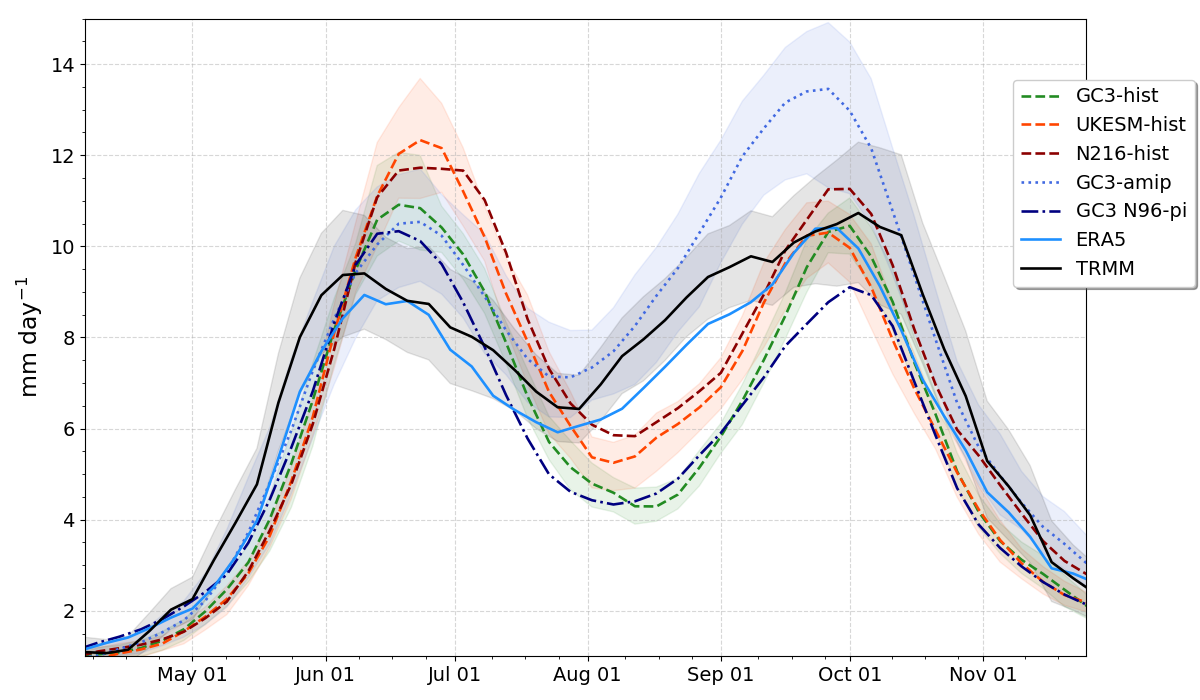
\includegraphics[width=\linewidth]{figures/seasonal_cycle_p3.png}
\caption{Pentad-mean precipitation in southern Mexico and northern Central America [95-86$^\circ$W,11-19$^\circ$N]. The shading for the TRMM dataset is a meausre of observational uncertainty obtained by bootstrapping the interannual variability 10000 times whereas the shading for the CMIP6 experiments show the ensemble spread where multiple ensembles where available. }
\label{fig:msdcaribb}
\end{figure} 
 
  Therefore, the purpose of this chapter is to examine previously proposed physical mechanisms for the MSD in the ERA5 reanalysis and the MOHC submissions to CMIP6. The focus of the chapter is on the region of Mesoamerica, i.e., southern Mexico and Central America, whereas the Caribbean MSD is not directly addressed in this chapter.

The previous chapter provides a useful diagnostic tool to separate the different stages of the MSD, a wavelet transform method (WT) that diagnoses the onset and end of the rainy season, as well as the start and end of the MSD. Similarly, the WT method can provide a robust measure of whether a given year and/or grid-point exhibits a robust bimodal signal. This chapter will use the WT method to separate the different stages of the MSD to better understand how the regional dynamics and thermodynamics varies from one stage of the seasonal cycle to the next. 

The remainder of this chapter is presented as follows. Section 2 describes the observational data and the CMIP6 experiments used in this chapter and a general overview of how the WT method is implemented and data is analysed. Then, section 3 evaluates the seasonality and general representation of the key features of the regional climate.
Then, several previous hypotheses are tested in the simulations and contrasted against the reanalysis/observations. 
The roles of the East Pacific SSTs (section 4), cloud-radiative feedbacks (section 5) and the CLLJ and moisture transport (section 6) have been highlighted in the literature and are investigated with detail in the rest of the chapter.
  
 % , particularly of the simulated processes that cause the sub-seasonal variations of precipitation  as well as the differences between experiments with varying forcing and different horizontal resolution will also provide relevant information about the simulated current and future response to greenhouse forcing as well as highlight relevant biases in the region for model development. 





Convective quasi-equilibrium (CQE) and moist static energy (MSE) budgets have been succesfully implemented in monsoon regions to understand mechanisms that drive precipitation changes. The remaining section of this chapter uses MSE and CQE diagnostics to evaluate the role of thermodynamics and ascent within the moist column of the MSD for the seasonal changes to precipitation. 


\section{Data and methods}

\subsection{Observations and reanalysis data}

All the data used in this chapter is described in chapter \ref{ch:3-methods}. In particular, this chapter relies on the precipitation datasets of TRMM and CHIRPS, as well as the precipitation derived from ERA5. The rest of diagnostics are from ERA5 and unless otherwise specified the diagnostics were downloaded at the 0.75$^\circ$ resolution.

\subsection{CMIP6 data}

This chapter uses the output from the realizations of the HadGEM3 GC3.1 run at two resolutions at N96 and N216 and from UKESM1. These experiments described in section \ref{sq:cmip6exp}. This chapter follows the terminology and acronyms outlined in section \ref{sq:cmip6exp}. 

\subsection{Determination of the timings of the MSD}

 \begin{figure}[t!]
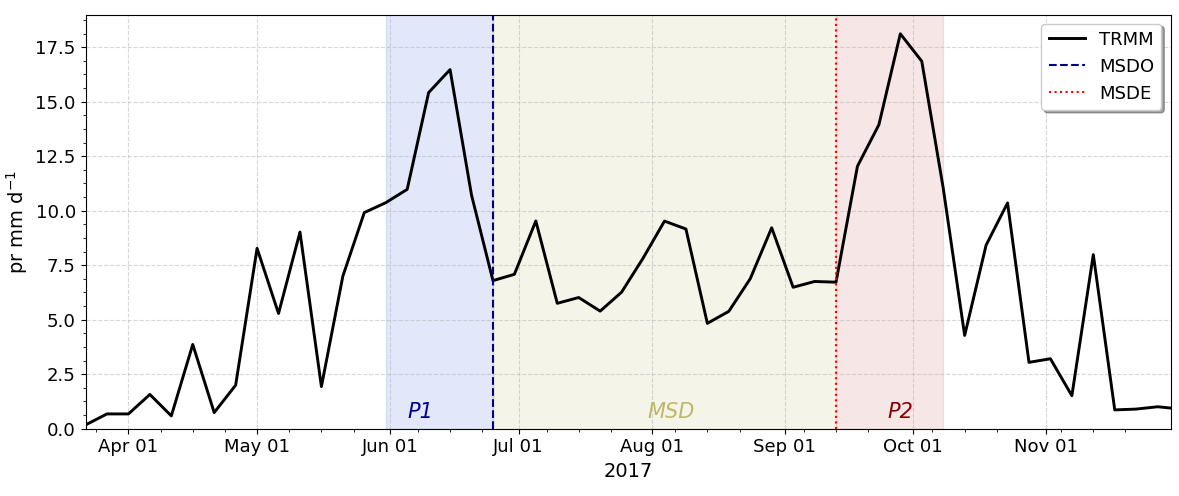
\includegraphics[width=\linewidth]{figures/explain_fig_msd.png}
\caption{Pentad-mean precipitation the study region [95-86$^\circ$W,11-19$^\circ$N] in the TRMM dataset for the summer of 2017. The timings of the onset (MSDO) and end (MSDE) of the MSD, as well as the first (P1) and second (P2) peak periods and the MSD periods are highlighted. }
\label{fig:explain_msd}
\end{figure}

Chapter 5 describes a wavelet transform (WT) method that can determine the timings of the MSD in observational gridded datasets, reanalysis and climate model precipitation time-series. 
This chapter uses the WT method to determine the onset (MO) and retreat (MR) of the monsoon rainy season, as well as the onset  (MSDO) and end (MSDE) of the MSD. 

As a brief reminder of the method, MO and MR are determined by the maximum and minimum sum of WT coefficients computed from a dilation scale vector ranging from 24 to 54 pentads. After MO and MR are determined, a second WT is computed with dilation scales to 10 to 24 pentads and the minimum sum of the WT coefficients corresponds to the onset of the MSD and the maximum to the end of the MSD (MSDE). 
Similarly, the timings of the first (P1) and second (P2) peaks of precipitation are determined from the results of WT method: P1 is defined as the period between the MSDO and the preceding 4 pentads or 20 days, whereas the second peak is defined as the period between the date of MSDE and the subsequent 4 pentads. An example of this separation of the MSD timings for each year is given in Figure \ref{fig:explain_msd}, for precipitation observed from TRMM in 2017 over the study region.

The area of study of this chapter is in southern Mexico and northwestern Central America (depicted in Figure \ref{fig:model_pr}) a region where Chapter 5 showed to exhibit robust and strong MSD signals. The WT method was implemented on the TRMM, CHIRPS and ERA5 datasets and in the model output over the precipitation time-series area-averaged over the study region. 


\section{Climatological features}

\label{sq:msdclim}



The seasonal cycle of precipitation in the region of interest (Figure \ref{fig:msdcaribb}) is reasonably well simulated by several experiments of GC3, N216 and UKESM1 and by ERA5.
The two-peak structure of the MSD is observed in TRMM and ERA5 as two precipitation maxima, the first peak found during early to mid-June and the second peak at the end of September, separated by a drier period that spans from late June to late August. The precipitation in ERA5 not only closely follows the precipitation variations at the pentad scale but also generally agrees with the magnitude of precipitation during the first peak, the MSD and second peak periods.
The MSD in the experiments is observed one or two pentads after TRMM and ERA5 (see the mean values in the previous chapter) and shows a stronger variation of precipitation between the first peak and the Midsummer. 
In general, the pre-industrial control experiments show a higher magnitude of precipitation during the first peak and the MSD period whereas GC3-amip experiments are characterized by a wetter second peak. 

  \begin{figure}[t!]
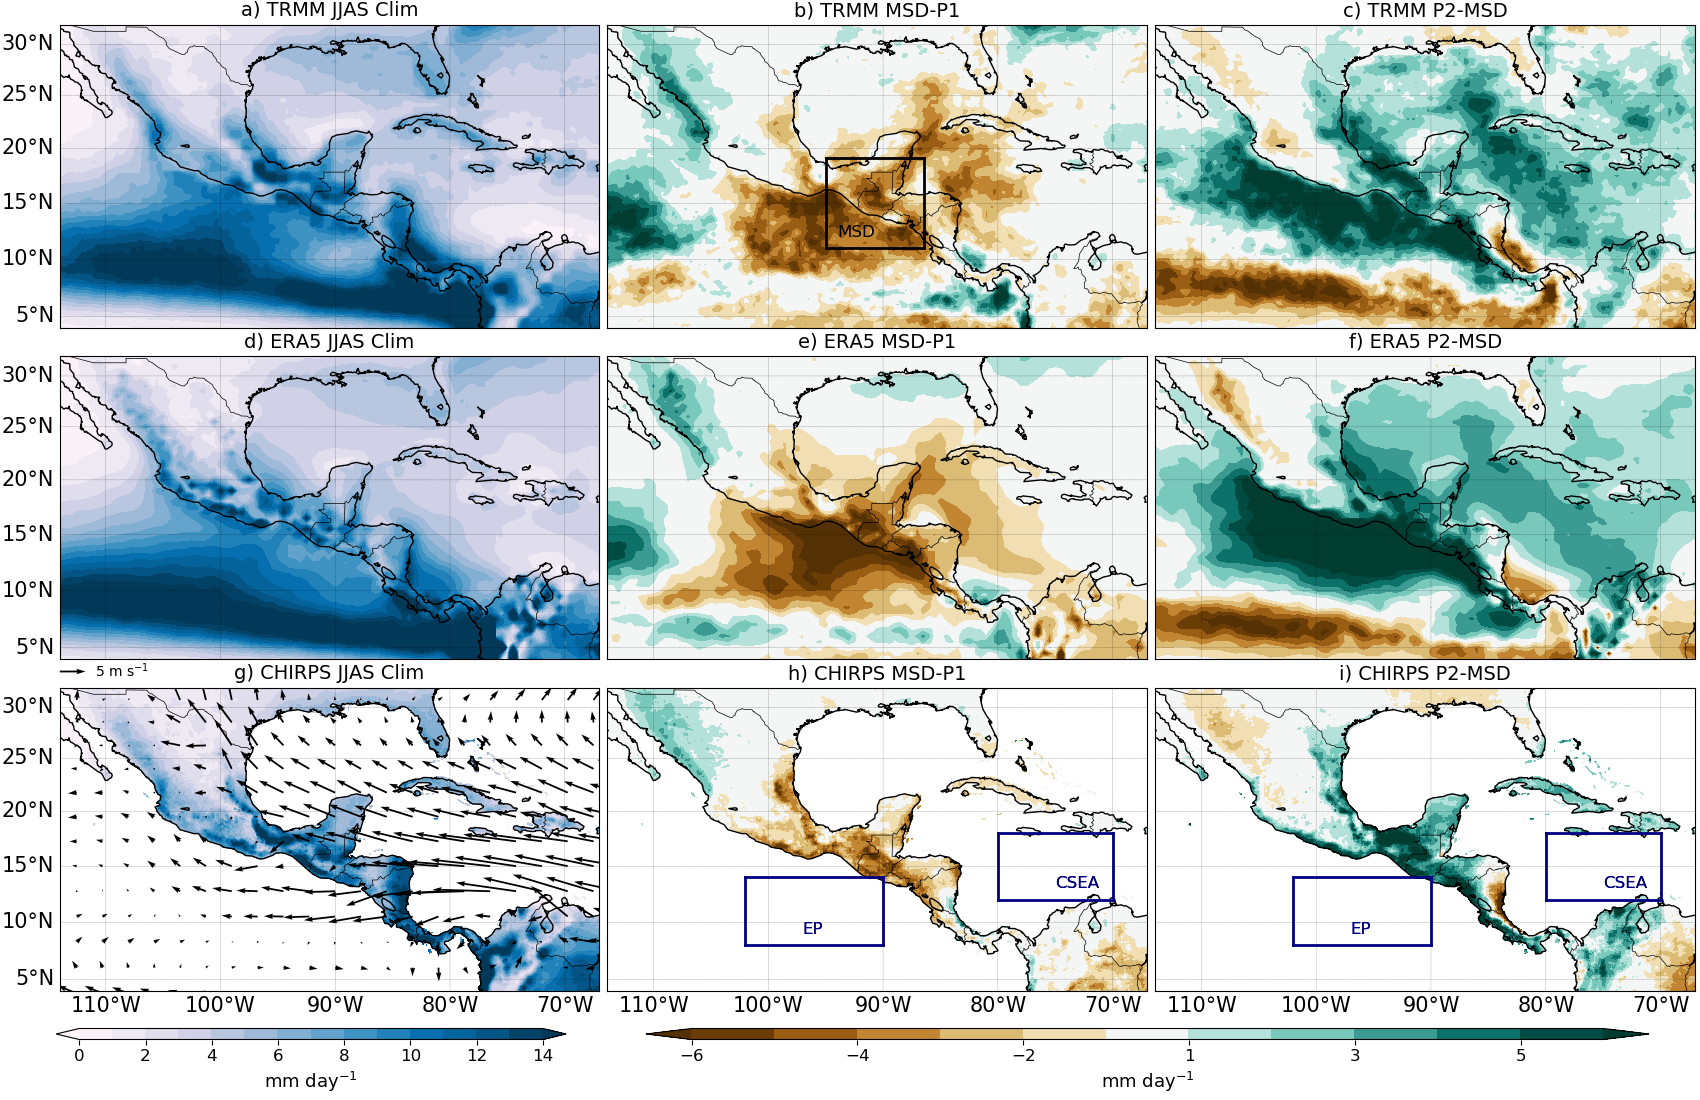
\includegraphics[width=\linewidth]{figures/fig2obs_prdiff_2.png}
\caption{ (a, d, g) Climatological JJAS rainfall and the difference between  (b, e, h)  the midsummer drought and the first peak periods and (c, f, i)  between the second peak and the midsummer drought periods for (a-c) TRMM, (d-f) ERA5 and (g-i) CHIRPS. The climatological low-level winds (at 850 hPa) for JJAS in ERA5 are shown in c). }
\label{fig:eof2}
\end{figure} 
 



The simulated spatial distribution of the climatological rainfall and the rainfall anomalies associated with the MSD in ERA5 agrees well with TRMM and CHIRPS (Figure \ref{fig:eof2}). The simulations reasonably capture rainfall in the regions over land with maximum precipitation rates in the Mexican states of Campeche, Veracruz and Chiapas, as well as in Guatemala and in the East Pacific Ocean. ERA5 shows stronger precipitation differences between the MSD stages, as rainfall in the East Pacific region in ERA5 varies by more than 5 mm day$^{-1}$ between the first peak, the MSD and the second peak. In turn, the simulations (Figure \ref{fig:model_pr}) have important biases in the magnitude of the  precipitation in the East Pacific ITCZ with a positive bias of 3-6 mm day$^{-1}$ depending on the simulation as well as a dry bias over southern Mexico and Central America, documented in chapter \ref{ch:4-ams}


\begin{figure}[t!]
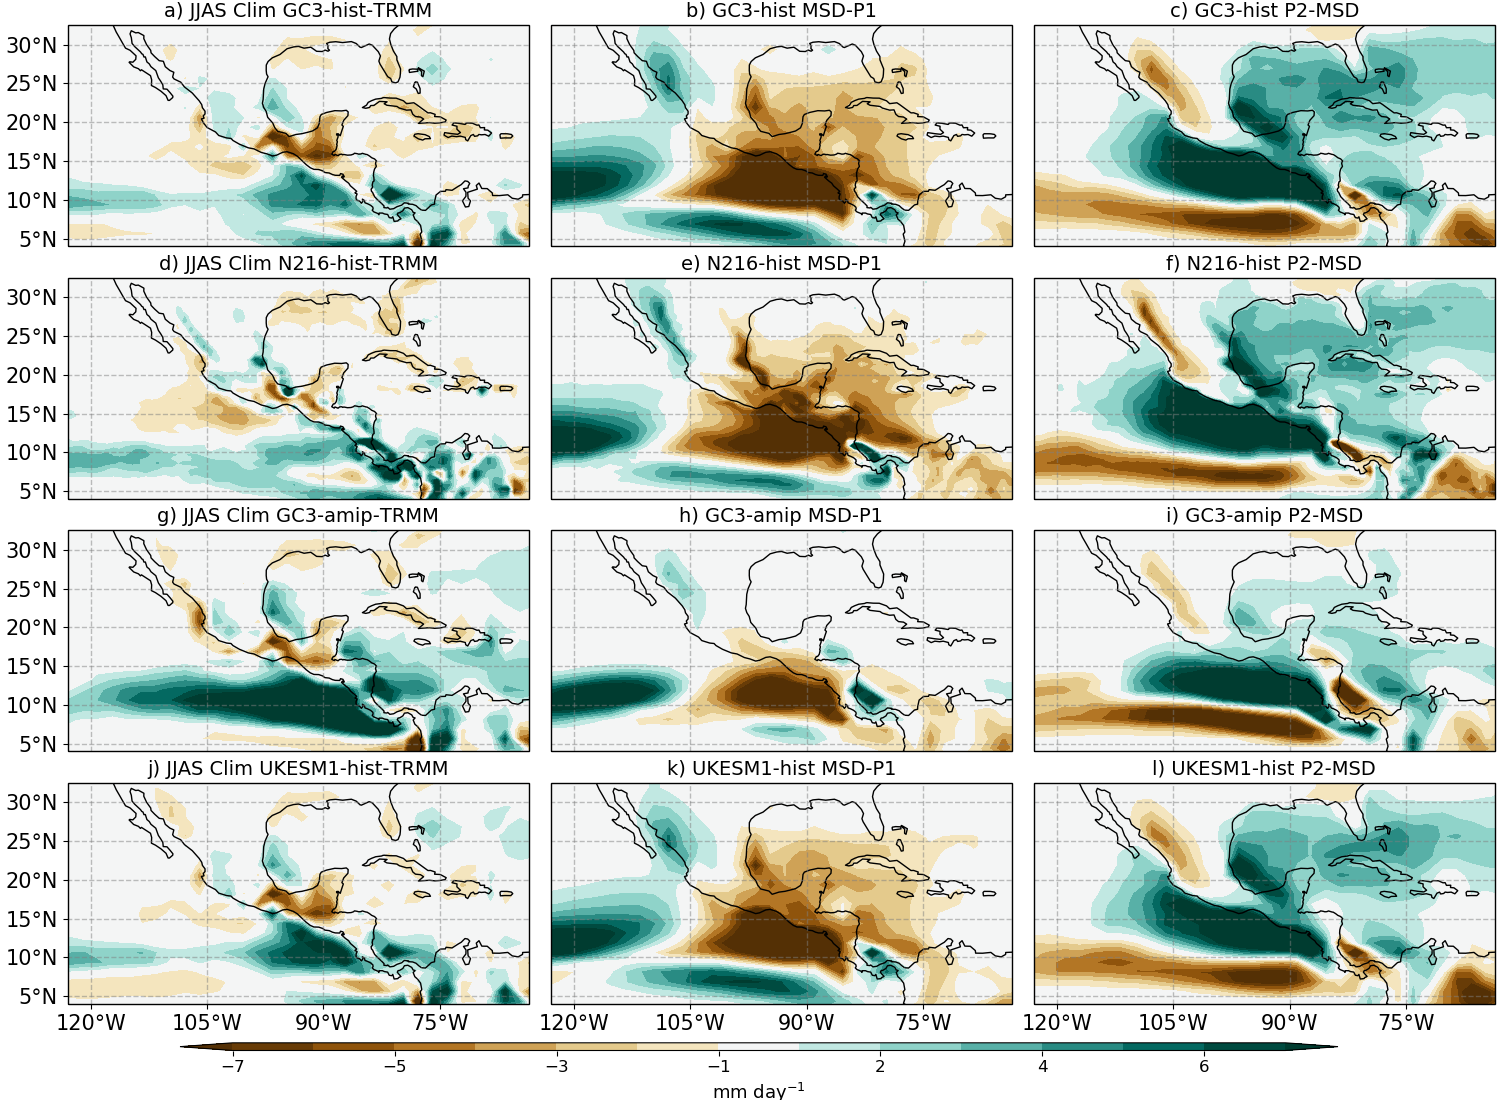
\includegraphics[width=\linewidth]{figures/fig2obs_prmodels3}
\caption{ (a, d, g, j) JJAS model bias compared to TRMM and the difference between  (b, e, h, k)  the midsummer drought and the first peak periods and (c, f, i, l)  between the second peak and the midsummer drought periods for four different simulations.}
\label{fig:model_pr}
\end{figure} 
 
The simulations capture the spatial patterns of the variations associated with the MSD stages.
  In observations and reanalysis (Figure \ref{fig:eof2}), the MSD variations have regional scales since even though the timings used to compute the composite difference between the MSD periods were computed using a time-series averaged over the study region, the precipitation differences spread south to the easternmost Pacific Ocean but also east to the Caribbean sea and into the northeastern Mexican states. The simulations also exhibit similar regional-scale patterns of precipitation differences both for the MSDO-MSD and the MSDE-MSD panels, though the precipitation differences associated with the MSD over the ocean in the models are notably larger than in the observations and reanalysis.  
 
 
 
\label{sq:msdclim}
 \begin{figure}[t!]
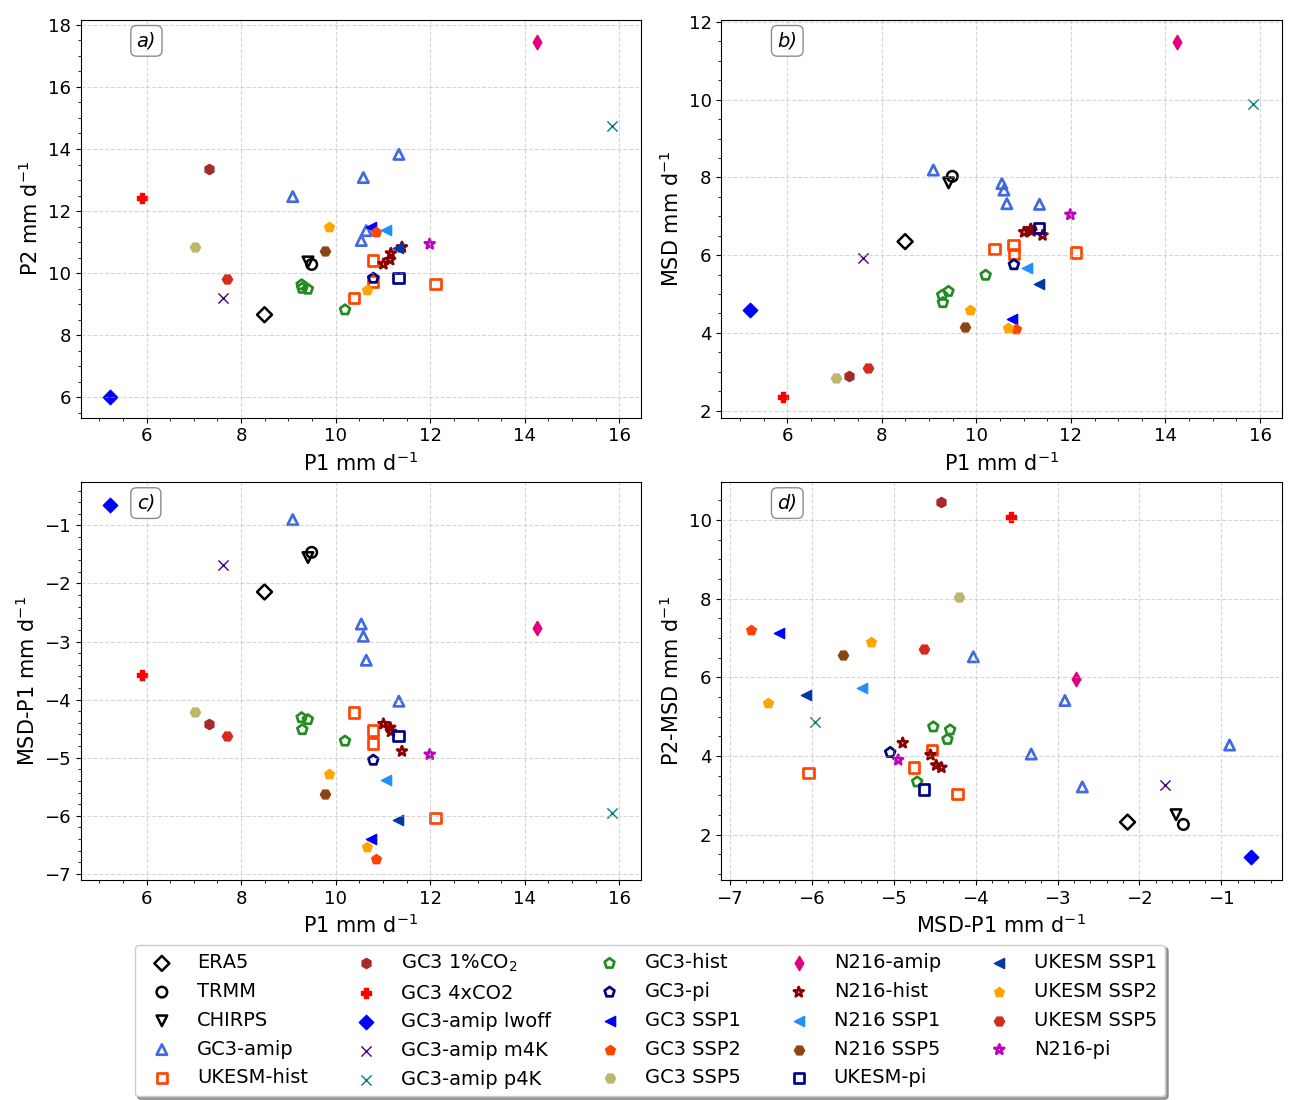
\includegraphics[width=\linewidth]{figures/dumscatter_2.png}
\caption{(a, b) Scatter plots of the mean values of precipitation [mm day$^{-1}$] for TRMM, ERA5, CHIRPS and the experiments during the first peak (P1), the MSD and the second peak (P2) periods and (c, d) the precipitation differences between the three periods. 
  }
\label{fig:scatter_msd}
\end{figure} 

The mean rainfall observed in the three periods (P1, P2 and the MSD) in the simulations varied notably between model configurations and with external forcing (Figure \ref{fig:scatter_msd}).
 The scatter of the first and second peak and the MSD mean rainfall rates  shows, first, that the mean rainfall in each stage is not linearly related to another, i.e., a larger magnitude of the first peak of precipitation does not necessarily imply a wetter or drier MSD period. The atmosphere-only run, GC3-amip, is a good example of this behaviour as the mean rainfall during P1 is roughly the same as in the rest of the simulations but the mean rainfall during the MSD is slightly larger than in the rest of the simulations and the P2 precipitation is largest in GC3-amip. 
 
 
Second, the magnitude of the first decrease in rainfall (MSD-P1) and the late-summer increase (P2-MSD) also show a significant spread amongst experiments, which also suggest that there is no clear association between the magnitude of the MSD and the magnitudes of the two peaks of precipitation in these simulations. The scatter of ERA5 in all panels is notably close to that of TRMM and CHIRPS, which is further evidence that the timings and strength of the MSD is well represented by this reanalysis.

 %In observation and reanalysis, the interannual variability shows a similar behaviour, i.e., the magnitude of precipitation at each stage is not related to the next stage (not shown). 

 \begin{figure}[t!]
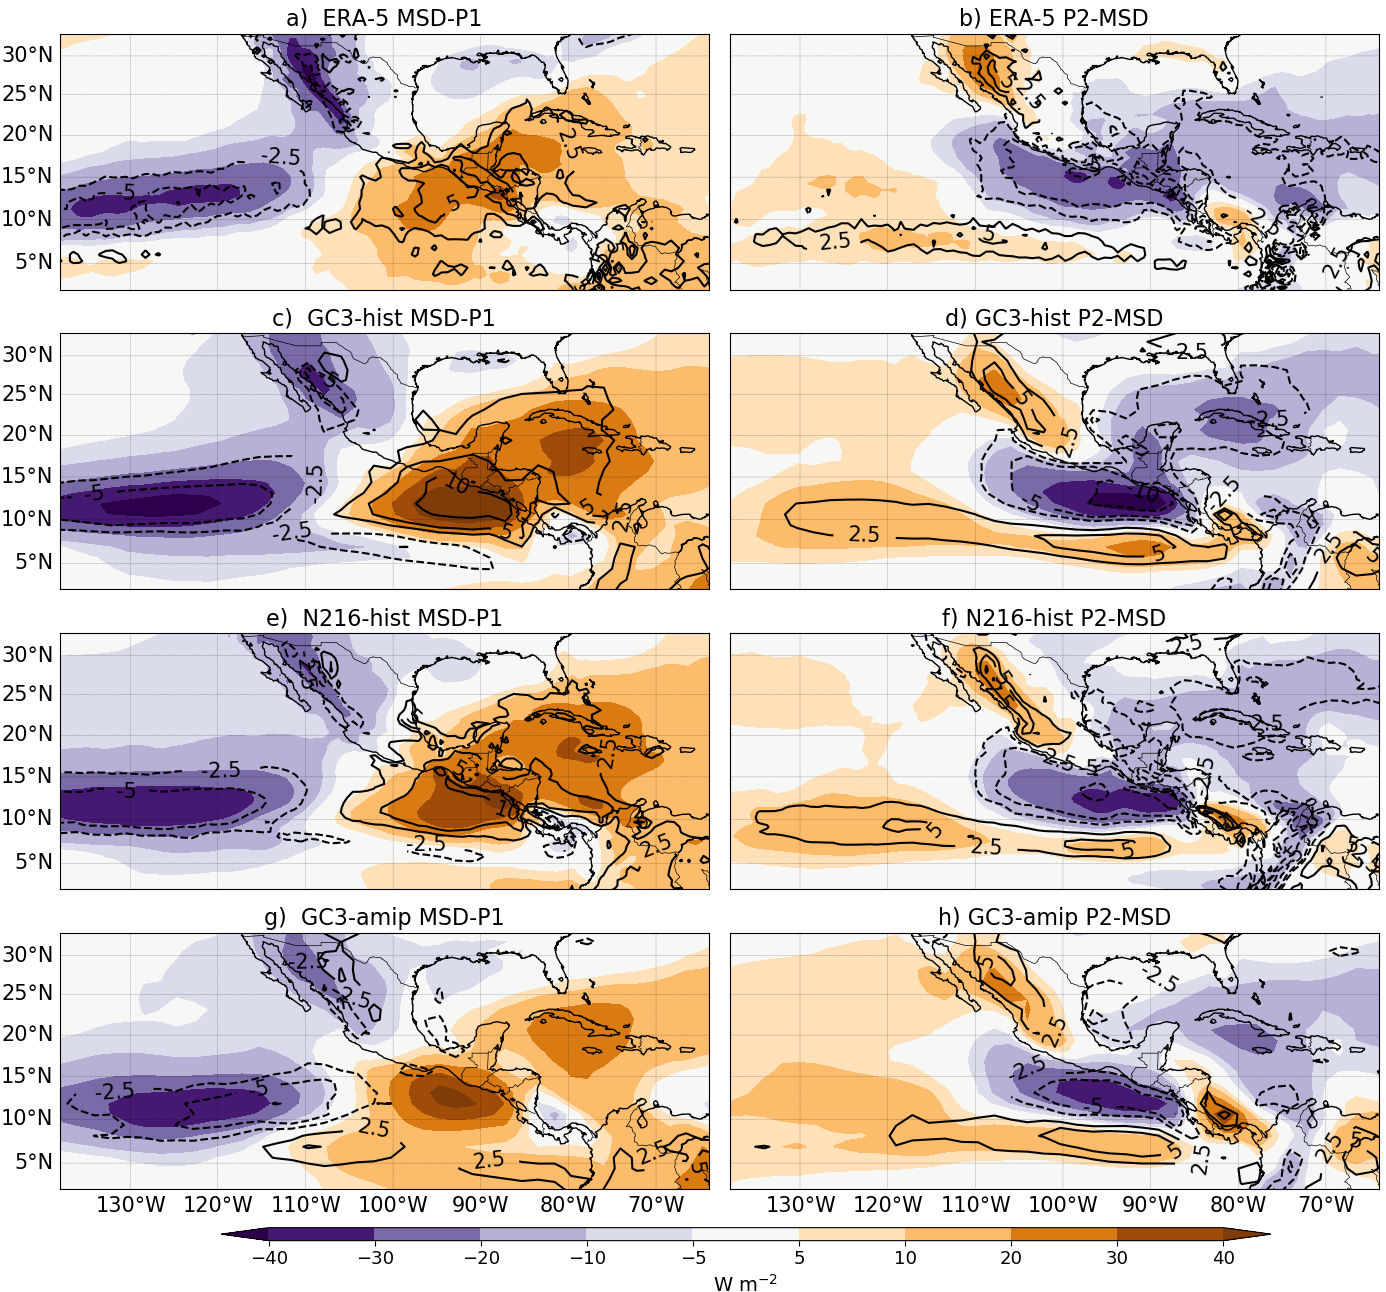
\includegraphics[width=\linewidth]{figures/fig4_olrv_3.png}
\caption{Outgoing long-wave radiation (OLR) [W m$^{-2}$] (shaded) and $\omega$ 500-hPa [$10^{-2}$ Pa s$^{-1}$] (line contours) differences between the MSD and MSDO and the MSDE and MSD.}
\label{fig:olranom}
\end{figure}

 The outgoing long-wave radiation (OLR) and vertical velocity ($\omega$ at 500 hPa) differences associated with the MSD (Figure \ref{fig:olranom}) also show that the MSD is not a local-scale feature but convective activity varies coherently in neighboring regions. From the MSDO to the MSD, OLR and $\omega$, increase notably in the easternmost Pacific, in southern Mexico and northern Central America and extend into the Caribbean islands and Sea; because $\omega$ is defined as $\omega=DP/Dt$  these positive anomalies are indicative of less deep convective activity and weaker convection. The OLR anomalies extend into the North Atlantic. 
 
 In contrast, a region several degrees west into the open Pacific Ocean (125$^\circ$W) and north of the study region into the North American monsoon region show signs of negative OLR and $\omega$ anomalies, in the MSD-MSDO panels, which are indication that simultaneously to the onset of the MSD,  convection is observed stronger and deeper in the North American Monsoon region and in the Pacific region west of the continent. The variations at around 125$^\circ$W where also found by \cite{herrera2015}. 
 
 \begin{figure}[t!]
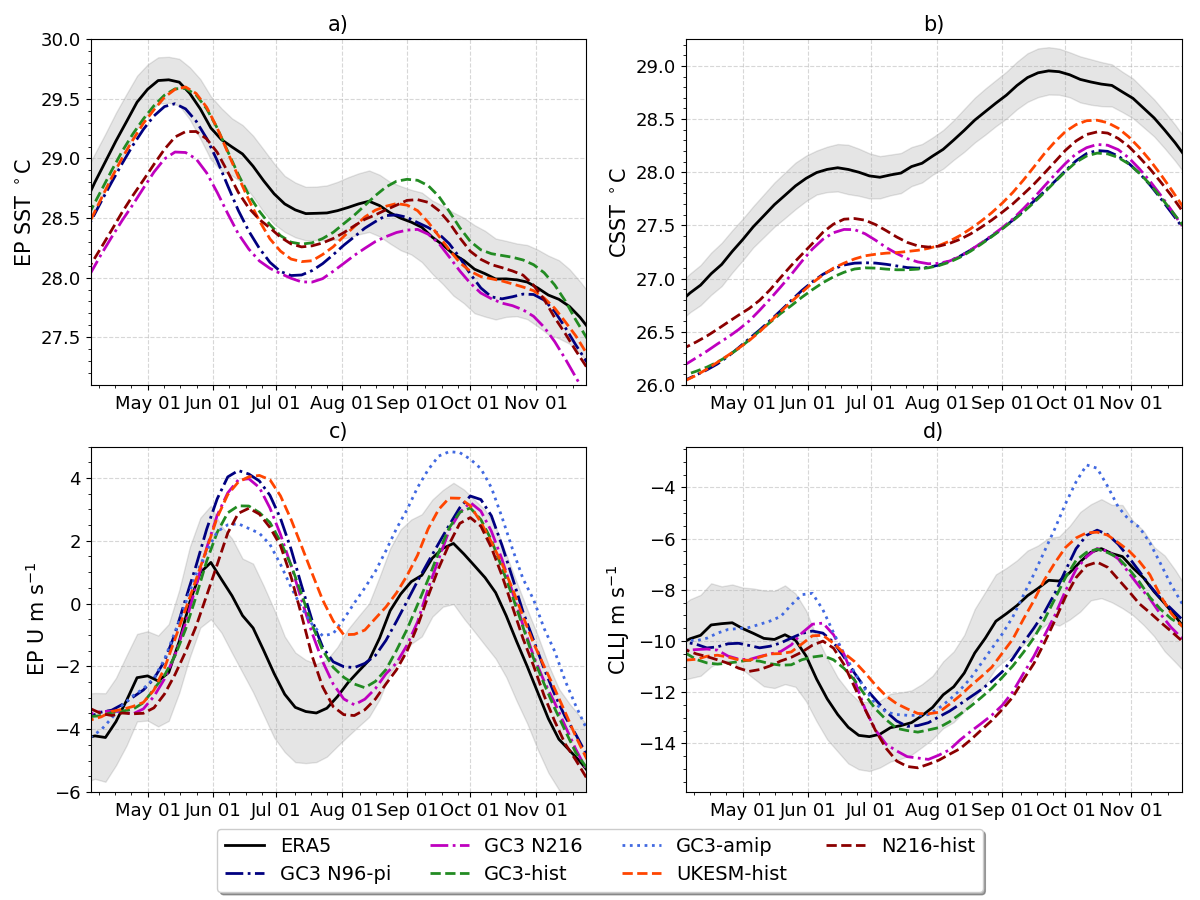
\includegraphics[width=\linewidth]{figures/index_seasonal}
\caption{Pentad-mean seasonal march of the (a, b) SSTs [$^\circ$C] and (c, d) the low-level (925-hPa) zonal wind flow [m s$^{-1}$] in (a) the easternmost equatorial Pacific and (b, d) the Caribbean Sea. The transparent shading is as in Figure \ref{fig:msdcaribb}.}
\label{fig:csst}
\end{figure}
 
 
 The OLR and $\omega$ variations associated with the end of the MSD (MSDE) show a relatively opposite picture to the MSD-MSDO differences. OLR and $\omega$ decrease all across the central and south western coast of Mexico and northern Central America extending into the Caribbean Sea whereas positive differences are found in the North American Monsoon region and in the Pacific Ocean at around 125$^\circ$W.  

Several climatological features of the region play key roles for the MSD, according to the various hypothesis in the region. The most prominent factors include the seasonal cycle of the East Pacific (EP) SSTs, the Caribbean Sea SSTs, and the Eastern Pacific wind flow and the CLLJ \citep{magana1999,amador2008,herrera2015,straffon2019,garcia2020sub}. 
The seasonal cycle of these features in ERA5 and the simulations (Figure \ref{fig:csst}) shows that the models are able to replicate the seasonal variations of the SSTs and the zonal wind flow of the region albeit some key biases. 

The seasonal cycle of EP SSTs show a maximum peak SST in late May, prior to the first-peak of precipitation in Central America. In contrast, the Caribbean SSTs peak in early fall, about five months later, during late September. After the peak SSTs in late, the EP SSTs decrease to a local minimum found in July both for ERA5 and the simulations. The models, however, show an overall cold bias in the SSTs in both regions, but this bias is most pronounced in the Caribbean Sea where throughout the wet season the SSTs in the models are lower than in ERA5. 

The CLLJ seasonal cycle is roughly replicated by the simulations, compared to ERA5, although the peak strength of the CLLJ found in ERA5 during the last week of June is delayed in the simulations by about 1 month, as the simulated CLLJ peaks in mid-July in all the simulations.
The low-level wind flow in the EP shows a bimodal regime in both ERA5 and in the simulations. 
The easterly flow in the EP during the spring becomes weaker turning positive at the end of May and reaching a local maximum in early June in ERA5 and mid-June in the simulations. This local maximum then decreases during June and early July as the zonal wind becomes easterly again and this easterly flow peaks in mid July in ERA5 and about three weeks later in the simulations. The strength of this easterly flow magnitude during the midsummer varies greatly amongst the simulations. 
After the midsummer easterly flow peak, or zonal wind local minimum, the zonal wind becomes westerly again peaking at the end of September-early August in both ERA5 and simulations. 



%Figure \ref{fig:eof2} shows the distribution of rainfall in the different stages of boreal summer in different CMIP6 experiments and ERA-5. 
%The main feature, the East Pacific ITCZ shows the maximum rainfall rates (>15 mm day$^{-1}$ in the models) and strong mid-level ascent (-0.1 Pa s$^{-1}$). Prior to the MSD, rainfall extends from the easternmost Pacific ITCZ into the North American continent. Therefore, the positive bias during the first peak over land is associated with the biased wetter EP ITCZ.  However, during the MSD, rainfall decreases over land remaining only above 10 mm day$^{-1}$ south west of the coastline in the models.

%The links between the EP and Caribbean SSTs and zonal wind flows, and the MSD precipitation are evaluated in the following sections to more detail.






\section{The East Pacific SSTs}

 

The East Pacific (EP) SSTs are the key element of the radiative convective feedback of \cite{magana1999} as the proposed feedback mechanism suggests that the summer march of the EP SSTs should also exhibit a bimodal signal, similar to that observed for precipitation but out-of-phase, with the SSTs leading the precipitation.
The EP SST seasonal cycle (Figure \ref{fig:csst}a) is characterized by peak SSTs in early May, and a subsequent cooling for the rest of the summer. 

According to the radiative convective feedback mechanism, the EP SSTs should be reduced prior to the onset of the MSD and then increase at the local minimum or rainfall or MSD period to enhance precipitation and cause the second peak of precipitation in late summer. However, in ERA5 the EP SSTs only very slightly increase during the MSD (Jul-Aug) and rather cool again in late August and September. In fact, the EP SSTs in ERA5 decrease after mid-August, in synchrony with the second peak in deep convection and precipitation. 
 In the models, however, there is indeed a second peak in EP SSTs but the timing of this peak is found in early September and nearly synchronous to the second peak in precipitation. The near synchrony of the second peak in EP SST and precipitation as well as the relatively small magnitude of the seconday summer increase in EP SSTs are not clear evidence that that the EP SSTs are leading precipitation from the drier MSD to the second peak of rainfall. 
 
 
%just prior to the onset date of rainfall. The EP SSTs decline during May in synchrony with the onset of rainfall (Figure \ref{fig:msdcaribb}) and the development of the first peak of rainfall and they stabilize during July and August and the SSTs  in ERA5. %Th which agrees with the notion that the first peak of precipitation is associated with the increased SSTs in the EP during late May. 




\begin{figure}[t!]
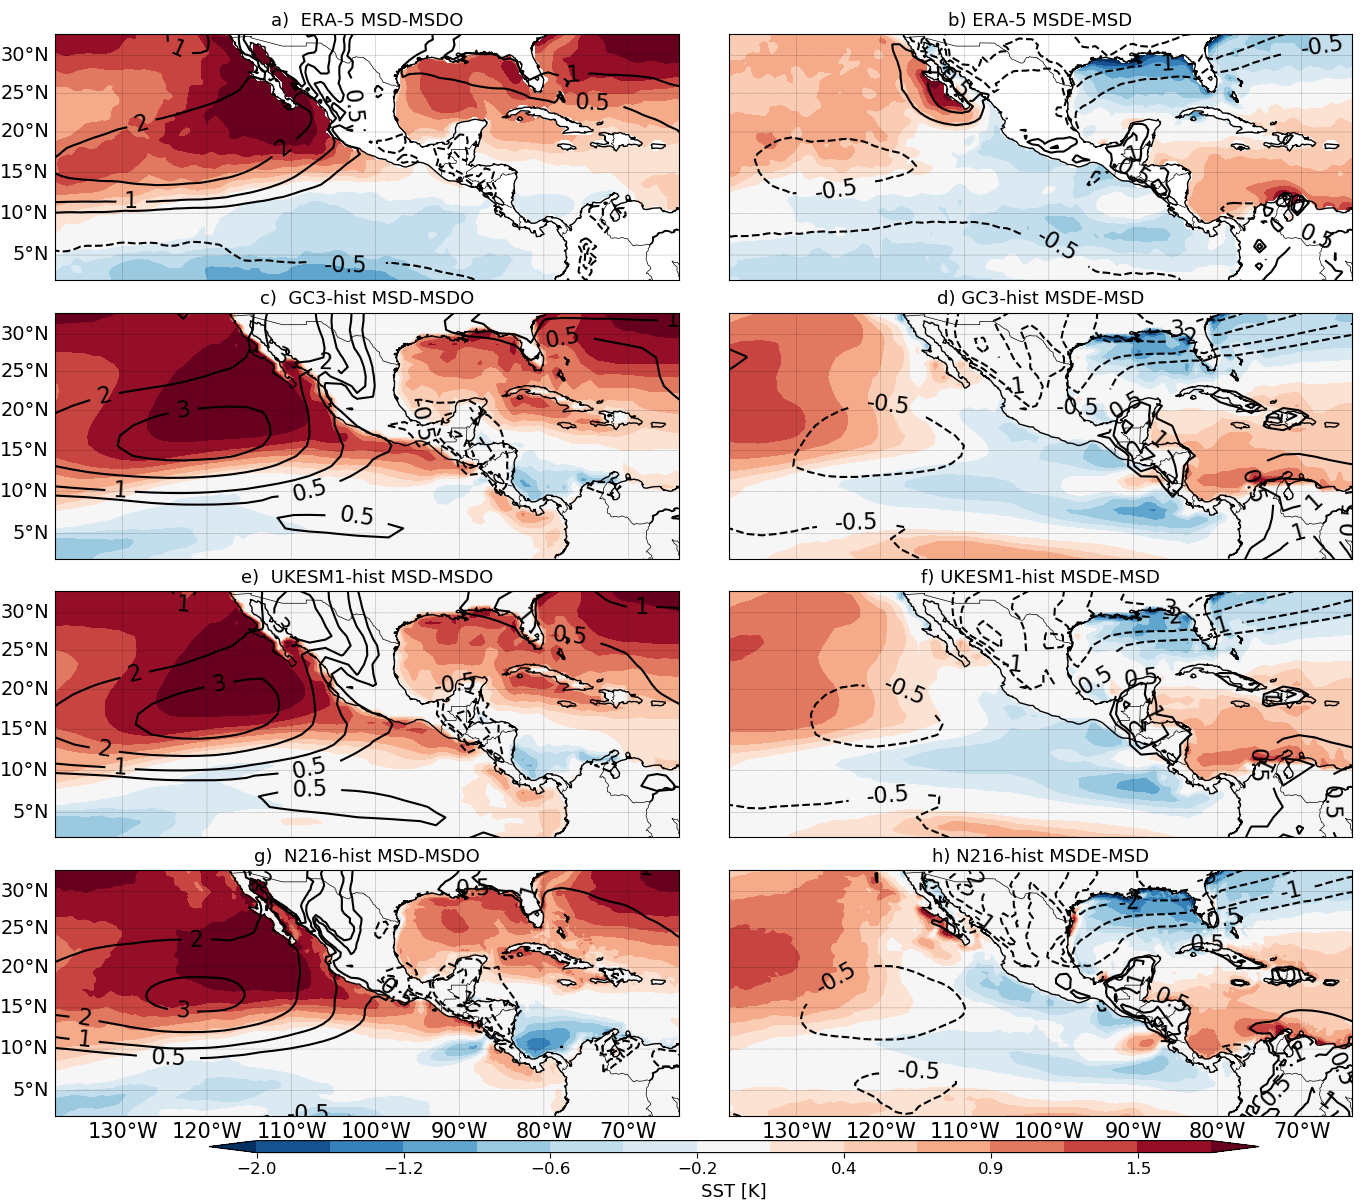
\includegraphics[width=\linewidth]{figures/fig4_sstv_3.png}
\caption{As in Figure \ref{fig:olranom} but the anomalies are shown for SSTs [K] (contours) and surface humidity [g kg$^{-1}$] (line-contours).  }
\label{fig:msdsstanom}
\end{figure}

% However, SSTs in the easternmost Pacific do not increase after, during or at the end of the MSD (Figure \ref{fig:csst}a). 



The spatial distribution of synchronous SST and surface humidity variations with the MSD timings  (Figure \ref{fig:msdsstanom}) suggests that little change EP SSTs between the first peak (P1) and the  MSD periods, whereas the difference between the MSD period and the second peak (P2) show that SSTs decrease at the end of the MSD. From the P1 to the MSD the most notable change is the warming of the northwester coast of Mexico and of the Gulf of Mexico.
From the MSD to the P2 period, the Caribbean SSTs increase, associated with the peak Caribbean SSTs  at the end of the summer (Fig. \ref{fig:csst}b).
The historical simulations generally agree with the composite differences of ERA5, with no appreciable warming in the EP region in the MSD-P1 panels, and cooling in the EP and the Gulf of Mexico and warming in the Caribbean Sea in the P2-MSD panels.




A direct implication of the feedback mechanism is that the SST variability would force the surface humidity and ultimately precipitation. The surface humidity in the EP, however, is largely unchanged (less than 0.5 g kg$^{-1}$) during the various stages of the MSD, even though precipitation varies notably during these periods. Instead, the greatest variations in surface humidity are observed west of Baja California from the P1 to the MSD, and this region of increased surface humidity extends into the North American Monsoon region. Similarly, at the end of the MSD, the most notable variations in surface humidity is the drying of the North American monsoon region.
 The surface humidity variations in the simulations also agree well with those of ERA5 and are very similar amongst the realizations.


\begin{figure}[t!]
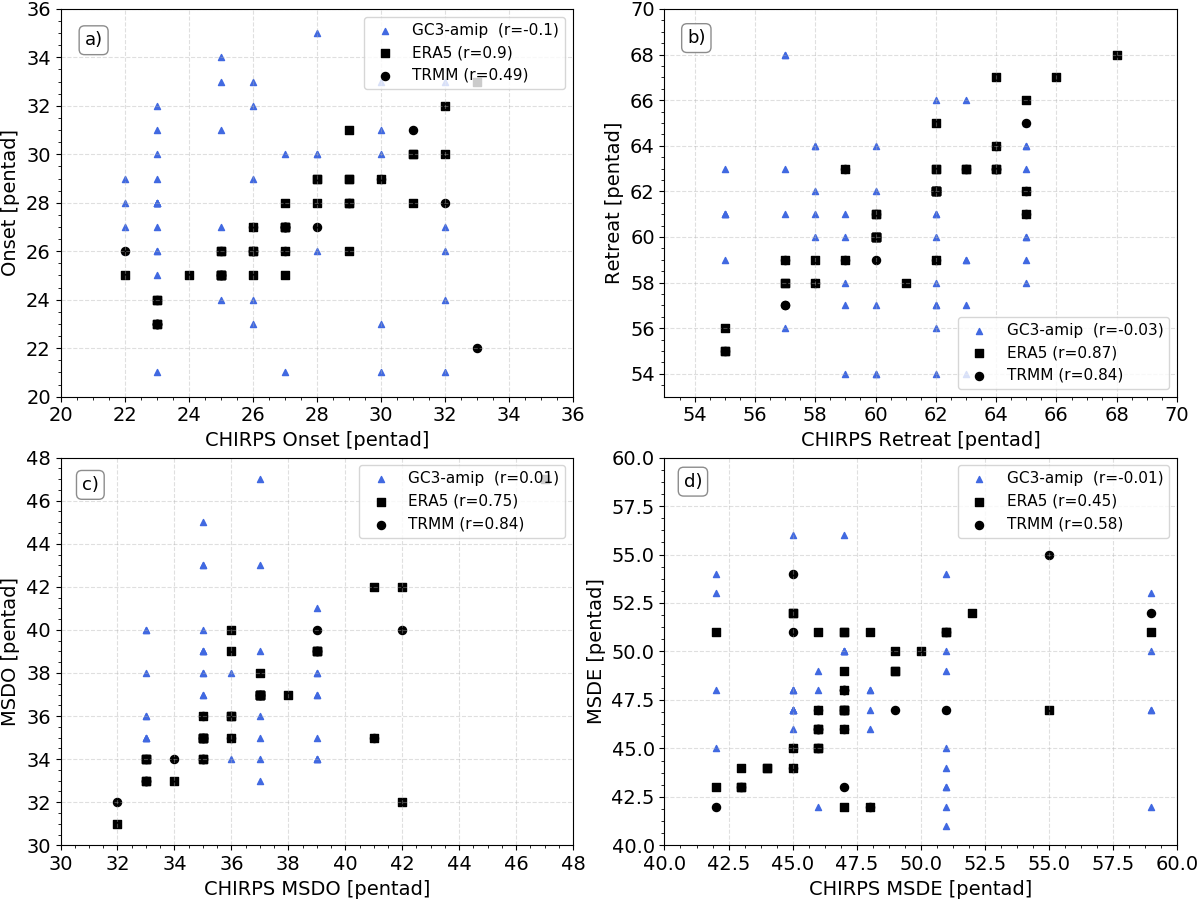
\includegraphics[width=\linewidth]{figures/master_sst_scatter.png}
\caption{Scatterplots of yearly timings in the MSD precipitation time-series diagnosed by the WT method for (a) monsoon onset (MO), (b) monsoon retreat (MR), (c) MSDO and (d) MSDE comparing the results of the CHIRPS dataset with ERA5, TRMM and the GC3-amip simulation. The legend shows the Pearson $r$ coefficient for each comparison. }
\label{fig:amipsstscatter}
\end{figure}



%The CLLJ is a strong easterly low-level (925 hPa) that reaches maximum winds speeds of 12 $m\,s^{-1}$ on February and July 
%The Caribbean Low-level Jet (CLLJ)is a strong low-level easterly jet in the Caribbean Sea that peaks at the end of June (Figure \ref{fig:csst}e) at the 925 hPa level \citep{amador2008,herrera2015,maldonado2016}. The CLLJ  determines the moisture transport from the Caribbean Sea into the eastern Pacific across the Central American landmass as well as the northward moisture transport into the Gulf of Mexico and Florida \citep{munoz2008,hidalgo2015,maldonado2016}.

If the EP SSTs play a dominant role in the timings and strength of the MSD, as implied previously \citep{magana1999,magana2005,herrera2015}, then the simulations that were run using observed-SSTs, i.e., the GC3-amip experiment, may be further explored to evaluate the links  between the timings or strength of the MSD in GC3-amip and ERA5. A scatter plot of the dates (pentads) of the MO, MR, MSDO and MSDE (Figure \ref{fig:amipsstscatter}) for matching years between the CHIRPS dataset and TRMM, ERA5 and the five ensemble members of GC3-amip show that the timings of the MSD in GC3-amip are unrelated to CHIRPS and ERA5, whereas ERA5, in spite of precipitation being largely a model-derived quantity in the reanalysis, produces MSD timings that agree fairly well with the CHIRPS and TRMM datasets. 
This evidence would suggest that the SSTs forcing the model in GC3-amip are not the dominant factor controlling the timings of the MSD in these atmosphere-only runs.

\begin{figure}[t!]
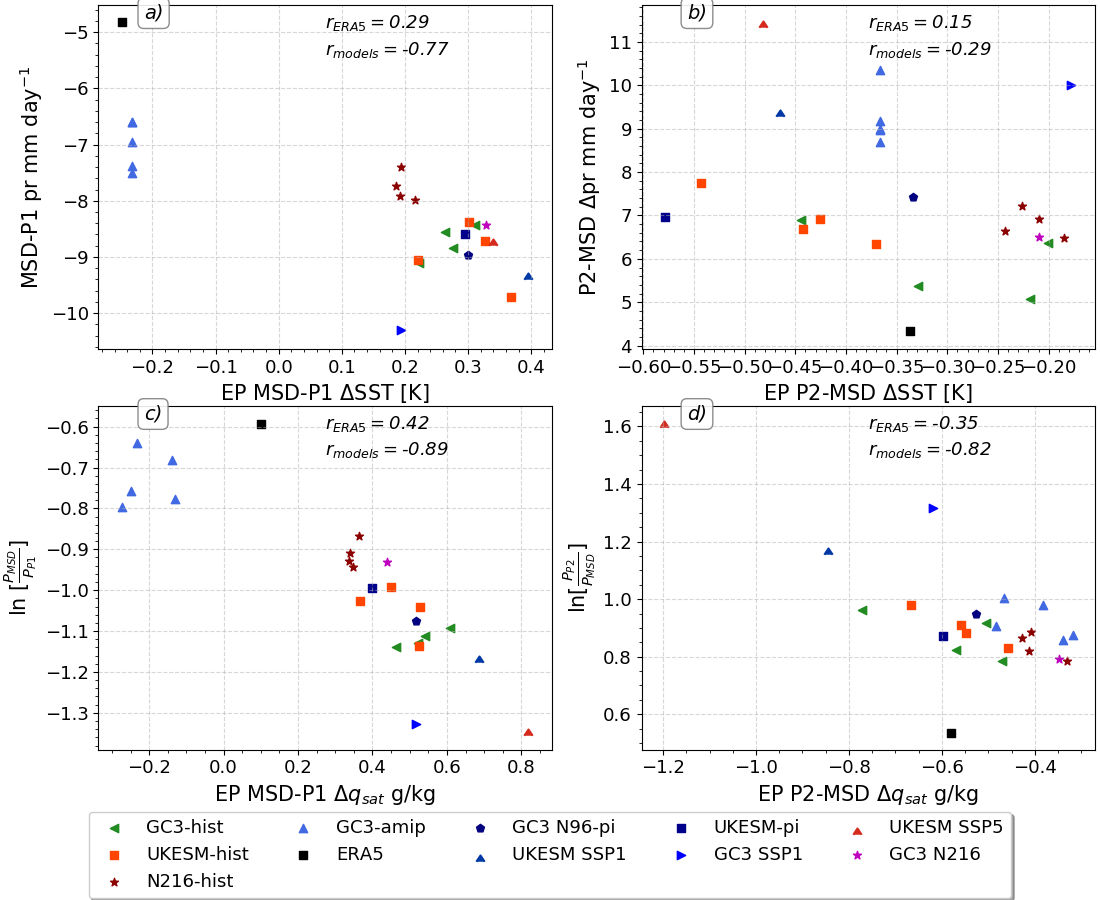
\includegraphics[width=\linewidth]{figures/sst_scatter_f.png}
\caption{Scatterplots of the mean changes in the East Pacific (a, b) sea-surface temperatures (SSTs) and (c, d) surface saturation specific humidity q$_{sat}$ in the x-axis with respect to precipitation variations in the MSD region on the y-axis for the (a, c) MSD-P1 and (b, d) P2-MSD periods.  The correlation coefficient of the interannual spread in ERA5 and the multi-experiment correlation coefficient are shown in each panel.   }
\label{fig:var_sst_lhf_scatter}
\end{figure}

%Figure \ref{fig:eof1} shows the climatological summer rainfall in the region and the difference in rainfall between the first peak and MSD and between the second peak and the MSD, characterised by the MSD-MSDO and MSDE-MSD differences. 
%Although the dates of the onset and end of the MSD determined using the WT method are defined using precipitation area-averaged over a relatively small region, the precipitation anomalies associated with the different stages of the seasonal cycle extend to most of Mexico and the Caribbean Sea and Gulf of Mexico. 
%For example, consider the MSDE-MSD differences in the CHIRPS dataset (Figure \ref{fig:eof1}i) where most of northern Central America, southern Mexico, the eastern coast of Mexico shows a positive (+5 mm day$^{-1}$) anomaly. In other words a large region experiences a relatively large increase in rainfall after the midsummer.

Alternatively, the interannual variability in ERA5 and the multi-experiment spread of the CMIP6 simulations may be further explored to understand whether the changes to the SSTs are related to changes in the precipitation in the MSD region. For this purpose, composite differences between the P1, MSD and P2 periods were computed for each variable for each year in each dataset and then averaged to provide a mean value of change associated with the timings diagnosed by the WT method.  For example, the mean difference in SSTs (Figure \ref{fig:var_sst_lhf_scatter}a) between the P1 and the MSD periods, show a cooling difference for ERA5, as for the GC3-amip experiments, but a positive difference (warming) for the coupled-model experiments associated (by construction) with a negative precipitation difference in the MSD region. 

The warming in the MSD-P1 difference (Figure \ref{fig:var_sst_lhf_scatter}a) in the coupled-model experiments agrees well with the seasonal cycle (Fig. \ref{fig:csst}) and suggests that in the model, as precipitation decreases during the MSD, the EP SSTs warm. At the MSDE, the EP SSTs cool (Figure \ref{fig:var_sst_lhf_scatter}b) associated with a positive increase in precipitation, suggesting an inverse relationship between EP SSTs and precipitation. However, the relationship does not seem to explain the inter-experiment spread or the inter-annual variability in ERA5 as the correlation coefficents are low and not significant. 

The feedback mechanism of \cite{magana1999} suggests that one of the main consequences of the SST changes should also be observed on the evaporation and surface humidity. Furthermore, evidence of tropical precipitation also suggests that the surface saturation specific humidity q$_{sat}$ is not only a measure of the capacity of air to hold moisture but can used to evaluate the sensitivity of precipitation to SSTs on seasonal time-scales \citep{yang2019,good2021}.

The temporal changes to $q_{sat}$ associated with the MSD timings (Figure \ref{fig:var_sst_lhf_scatter}c,d) are not positively related to changes in the precipitation over the MSD region. Although the inter-annual variability of $q_{sat}$ changes during the MSD-P1  period in ERA5 shows a positive correlation, the mean changes to $q_{sat}$ during this stage are very small compared to the differences in the experiments and, furthermore, the relationship for the simulations shows an opposite relationship (negative correlation). For the P2-MSD differences, there is a negative correlation for both ERA5 and the experiments. 

\begin{figure}[t!]
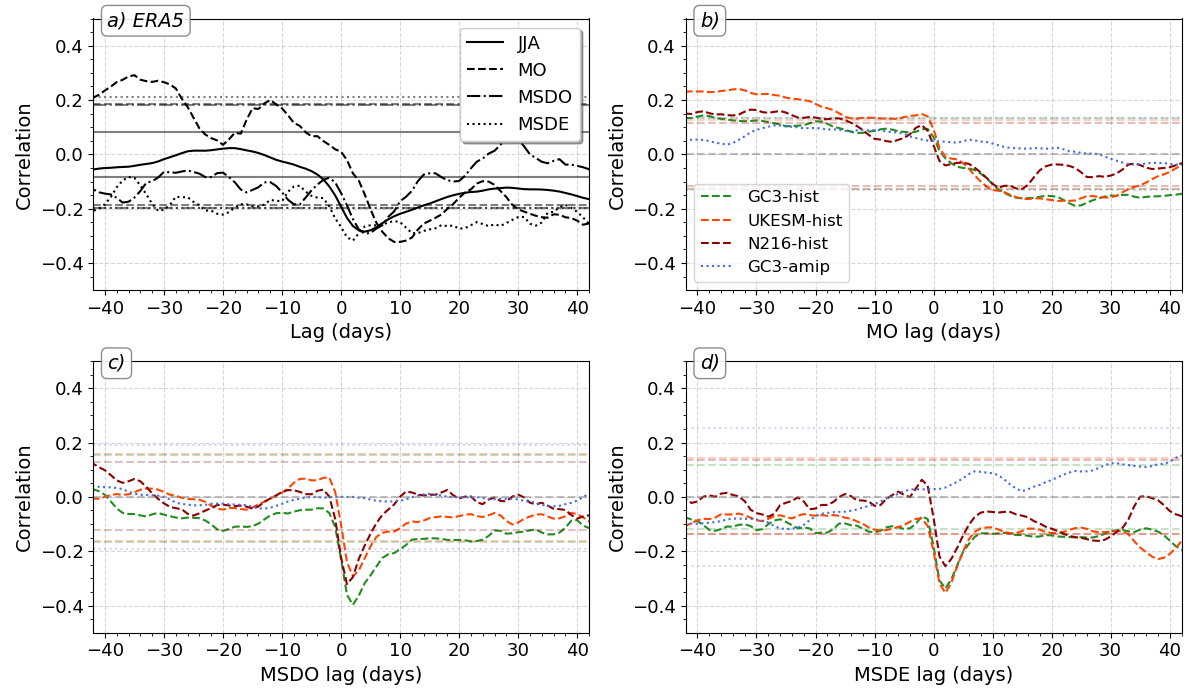
\includegraphics[width=\linewidth]{figures/sst_regg.png}
\caption{Lagged correlations between East Pacific SSTs and precipitation in the MSD region for (a) ERA-5 where the lag 0 date was used in four different ways: first, all the boreal summer JJAS SSTs and precipitation pairings, then lag 0 represents the monsoon onset (MO), MSD onset (MSDO) and MSDE dates. (b-d) as in (a) but for the simulations where the correlations are computed with the SST-precipitation timeseries lagged with respect to the b) monsoon onset date, the c) MSDO date and the d) MSDE date.   }
\label{fig:sst_lag}
\end{figure}

The previous results have analysed synchronous changes between the EP SSTs, surface humidity and $q_sat$ but the expected relationship may a lead-lag relationship, and as suggested by the radiative-convective feedback mechanism the SSTs should be leading precipitation. 
Lag-lead correlations (Fig. \ref{fig:sst_lag}) of the EP SSTs and the precipitation in the MSD region show that only during monsoon onset are these two fields significantly positively correlated at lags of $\approx$-35 days in ERA5 and -40 to -20 days in the historical experiments. In ERA5, the correlation for all the boreal summer (JJAS) sample is not significant in the SSTs leading  precipitation region and is only significant (negative correlation) at lag +5 days, indicative of an inverse SST-precipitation relationship where the SSTs follow precipitation. 
%SST response to positive precipitation increases.

In the models (Fig. \ref{fig:sst_lag}b-d), very similar results are shown as significant positive correlations at negative lags, indicative of SSTs leading precipitation, are only found for the MO panel, whereas for MSDO and MSDE, the correlations are only significant at a positive lag and for negative correlations, indicative of the precipitation leading the SSTs on the scale of 3-5 days.


%Biases in the strength and position of the EP ITCZ in Global Coupled Models (GCMs) \citep{bellucci2010,li2014,schneider2014} are a major reason for biases in the model representation of rainfall in Central America  \citep{rauscher2008}. 




%The CMIP6 Met Office models, HadGEM3 and UKESM1, are amongst the first models to simulate a bimodal regime in both Central America and Cuba (Figure \ref{fig:8}a and \ref{fig:msdcaribb}). 
%In Central America and southern Mexico, the models simulate a wetter-than-observed first peak of precipitation and a drier MSD period.
% 
%The so-called second peak of precipitation found in late August is simulated in close agreement with TRMM, except in the AMIP experiment which has a far too strong second peak mean precipitation rate.
% The seasonal cycle and other characteristics of the MSD showed noticeable differences between the different experiments analysed in this study. 

\section{On the role of cloud-radiative effects}

%\subsubsection{Climatological features of the MSD in UKESM1 and HadGEM3}
%Rainfall during the first peak has been too wet in these models since CMIP3, suggesting a persistent wet bias in this region associated with the East Pacific ITCZ \citep{ryu2014,mulcahy2018}. 

The mechanisms proposed by \cite{magana1999} and \cite{karnauskas2013} suggest that the net shortwave energy absorbed by the surface is key in the driving mechanism of the MSD. \cite{magana1999} suggests that tall convective clouds influence the timings and amount of this shortwave flux at the surface (SW), and although not explicitly mentioned as such, \cite{magana1999} argues that the cloud-radiative effects (CRE) experience seasonal changes that can explain the MSD. In turn, \cite{karnauskas2013} argues that the seasonal march of solar insolation characterized by the solar declination angle determines the net shortwave absorbed by the surface. These studies motivate a further inspection of cloud-radiative effects in the simulations to understand whether there is evidence to support previously proposed hypotheses.

Furthermore,  CRE effects have been shown to be very important for the timing and strength of regional \citep{guo2015} and axi-symmetric \citep{byrne2020} monsoons. The long-wave (LW) CRE plays an important role in the convective heating and moistening of the atmospheric column in tropical regions and the short-wave (SW) CRE affects the surface absorption of energy \citep{allan2011}. 
These studies motivate a deeper investigation of the CRE for the MSD timings and strengths in ERA5 and the simulations. The surface cloud radiative effect (CRE$_{surf}$) is computed from daily-mean fields following \cite{allan2011}, as the sum of the long-wave (LW) and SW CRE, i.e.:

\begin{multline}
CRE_{surf}=LW CRE_{surf} +SW CRE_{surf} \\ = LDS-LUS -(LDS_{cs}-LUS_{cs})+SDS-SUS-(SDS_{cs}-SUS_{cs})
\end{multline}

where the fluxes are depicted as long-wave (L) or short-wave (S) and downwelling (D) or upwelling (U) at the surface (S) and the suscript $_{cs}$ denotes under clear-sky conditions. The long-wave upwelling at the surface (LUS) cancels with the LUS$_{cs}$ because the long-wave emission from the surface is not dependent on the presence of clouds. The net CRE at the surface is then given by:

\begin{figure}[b!]
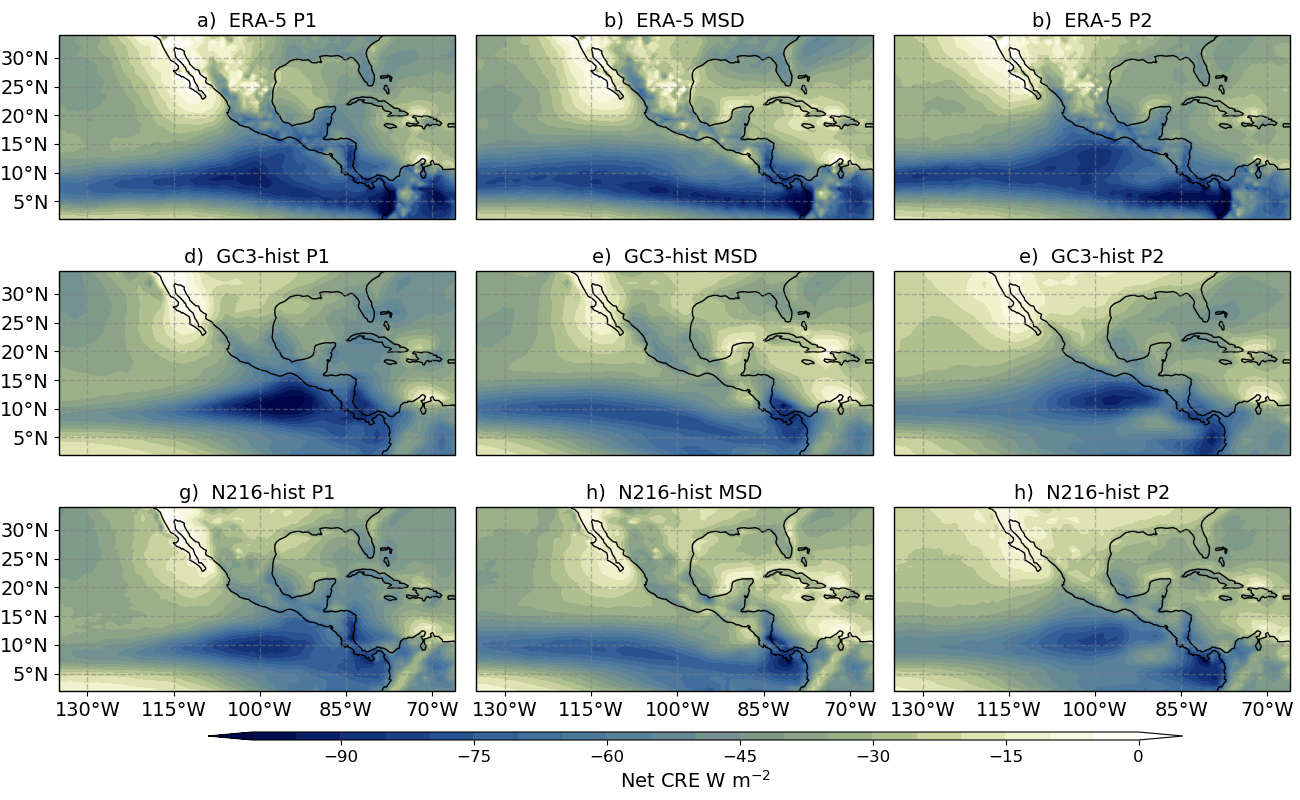
\includegraphics[width=\linewidth]{figures/fig4_creclim_3.png}
\caption{Composite mean cloud radiative effect (CRE) [W m$^{-2}$] during the periods of onset of the MSD, the MSD and the end of the MSD for (a-c) ERA5, and the ensemble mean of (d-f) GC3-hist and (g-h) N216-hist.}
\label{fig:cre_comp}
\end{figure}

\begin{equation}
CRE_{surf}=  LDS-LDS_{cs}+SDS-SUS-SDS_{cs}+SUS_{cs}
\end{equation}



The net CRE during P1, MSD and P2 periods (Fig. \ref{fig:cre_comp}) is negative  and the minimum are found at the East Pacific ITCZ region. The differences between the MSD timings closely follow the precipitation changes during these periods as the minimum CRE in the EP and the Mesoamerican region is found during the two peaks of precipitation with a reduced value over the continent and nearby coast during the MSD. The smallest CRE is found over the Baja California Peninsula. 
%During the MSD, the minimum in CRE is displaced west of the coastline into the region where the previous sections indicate increased convective activity.
The two historical ensemble means presented closely follow the results of ERA5, and the only notable difference between the lower (GC3) and the higher (N216) resolution historical experiments is that the CRE is stronger in GC3-hist during the P1 period than in N216-hist.

\begin{figure}[t!]
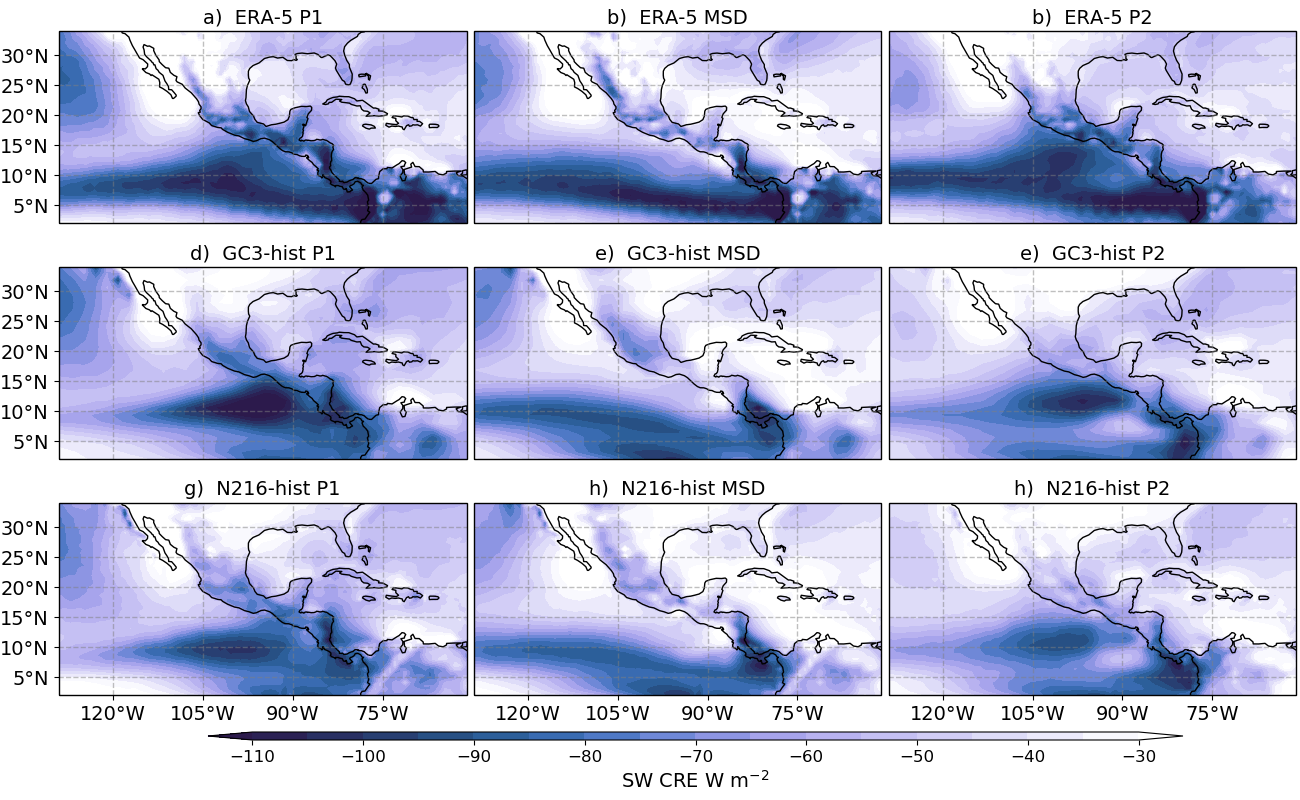
\includegraphics[width=\linewidth]{figures/fig4_swclim_3.png}
\caption{As in Fig. \ref{fig:cre_comp} but for the short-wave radiative effect.}
\label{fig:sw_comp}
\end{figure}

The individual contributions of the surface SW and LW CREs (Figures \ref{fig:sw_comp} and \ref{fig:lw_comp}) show that the dominant term in the EP and Mesoamerican regions is the SW term. The negative SW CRE is largest in the EP ITCZ region and the changes associated with the MSD timings are similar to those of the net CRE, i.e., in the MSD region the SW term in ERA5 during P1 and P2 is notably larger ($<-90$ W m$^{-2}$) than during the MSD.
The two historical experiments also show that the SW CRE is larger in magnitude in the EP ITCZ region and the show that the SW CRE over land varies notably from P1 to the MSD to the P2 periods.

In contrast, the LW term (Figure \ref{fig:lw_comp}), is generally smaller in magnitude than the SW CRE and is largest over land and in the ocean west of the California with little horizontal gradients over the EP region and the Caribbean Sea. 
The differences of the LW between the stages of the MSD are smaller than the SW term variations, but both in ERA5 and the simulations, the LW term over the EP and the Caribbean Sea is larger during the two peak periods than during the MSD. 

\begin{figure}[t!]
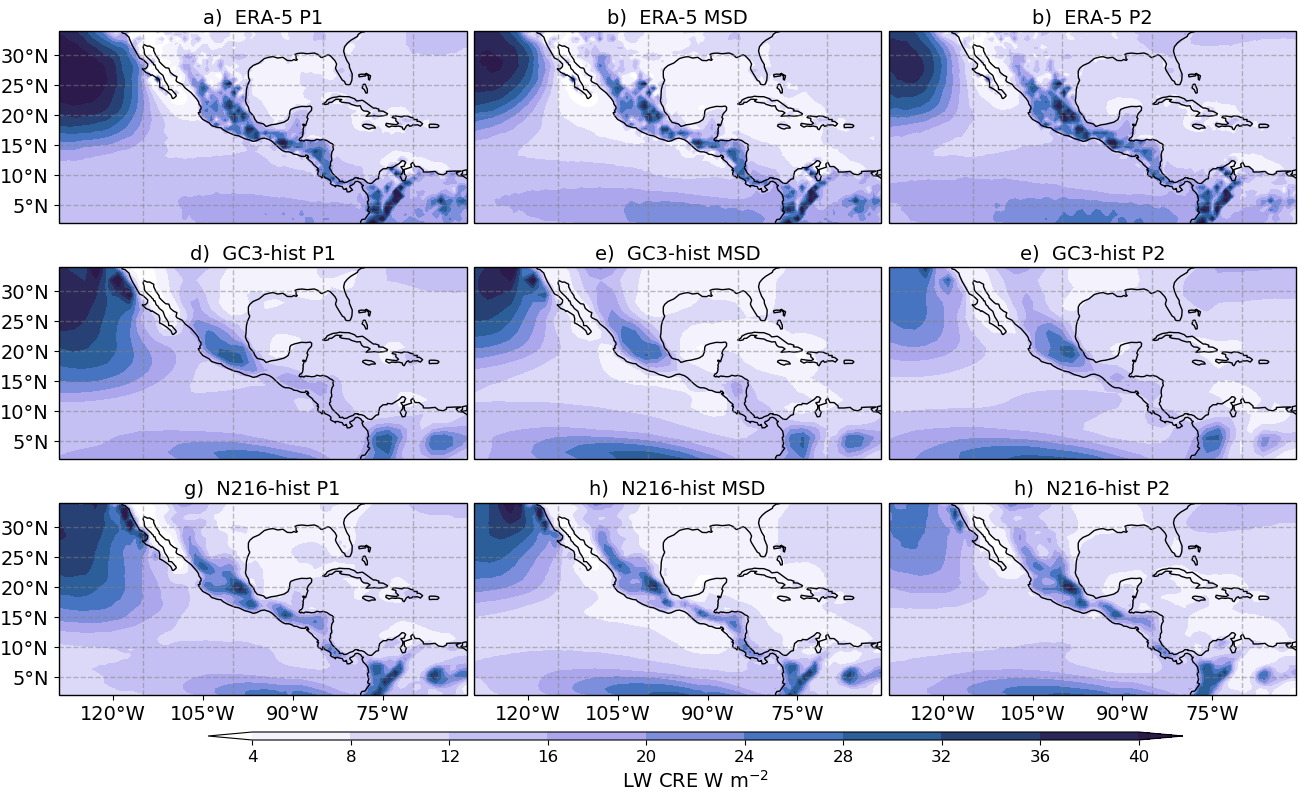
\includegraphics[width=\linewidth]{figures/fig4_lwclim_3.png}
\caption{As in Fig. \ref{fig:cre_comp} but for the long-wave CRE.}
\label{fig:lw_comp}
\end{figure}

These composites depict how the spatial distribution of the CRE varies with the MSD timings over the larger Intra-Americas Seas region, but how the seasonal variations in these terms actually changes in the MSD region is not obvious. The seasonal cycles of the SW, LW and net CREs (Figure \ref{fig:cre_seasonal}a-c) show bimodal signatures characterized by stronger CREs during the two peak periods during June and September and a relative minimum in between found in late July in ERA5 and early August in the simulations. 

The simulations reasonably simulate the magnitude of the net and SW CRE during the early summer season but overestimate the decrease in the net, SW and LW CRE during the midsummer, very likely associated with the underestimation of precipitation over this same period (Figure \ref{fig:msdcaribb}).

\begin{figure}[t!]
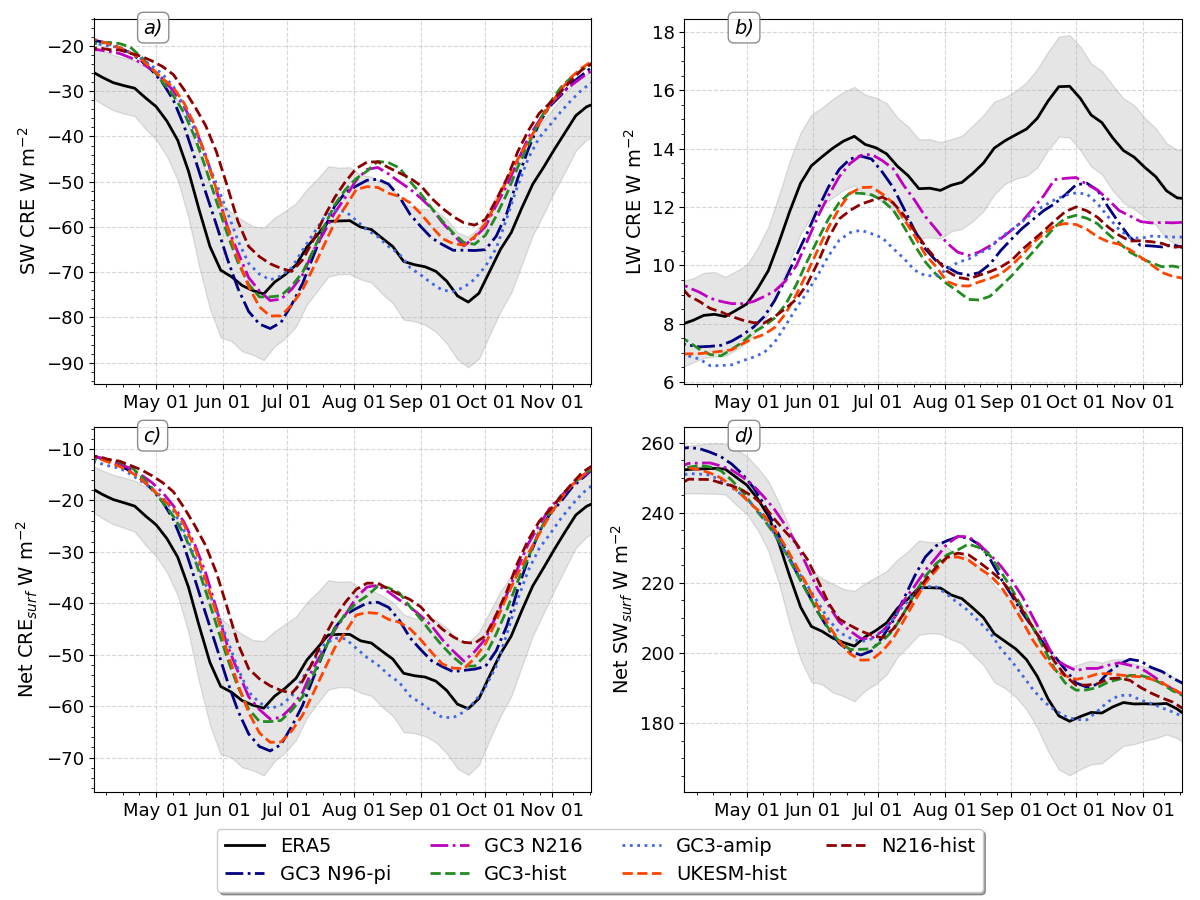
\includegraphics[width=\linewidth]{figures/cre_index_seasonal.png}
\caption{Pentad-mean seasonal cycle of the (a) SW and (b)  LW CREs, (c) the net CRE, and (d) the net SW at the surface, signed positive to indicate surface absorption of SW radiation.}
\label{fig:cre_seasonal}
\end{figure}

Both the theories of \cite{magana1999} and \cite{karnauskas2013} suggest that the net SW radiation absorbed at the surface is a key element of the MSD mechanism. Regardless of CREs, the net SW (the difference between upwelling and downwelling shortwave) absorption should also present a bimodal seasonal cycle.
In both ERA5 and the simulations the net SW (Figure \ref{fig:cre_seasonal}d) shows a bimodal local summer cycle characterized by a maximum peak in late May, which coincides with the peak in East Pacific SSTs. This peak in SW is followed by a local minimum during June which is followed by a secondary increase in July in ERA5 and extending to August in the simulations. After this second local maximum in SW, there is another sharp decrease in SW at the end of the summer, which coincides with the the second peak in precipitation. 

\begin{figure}[t!]
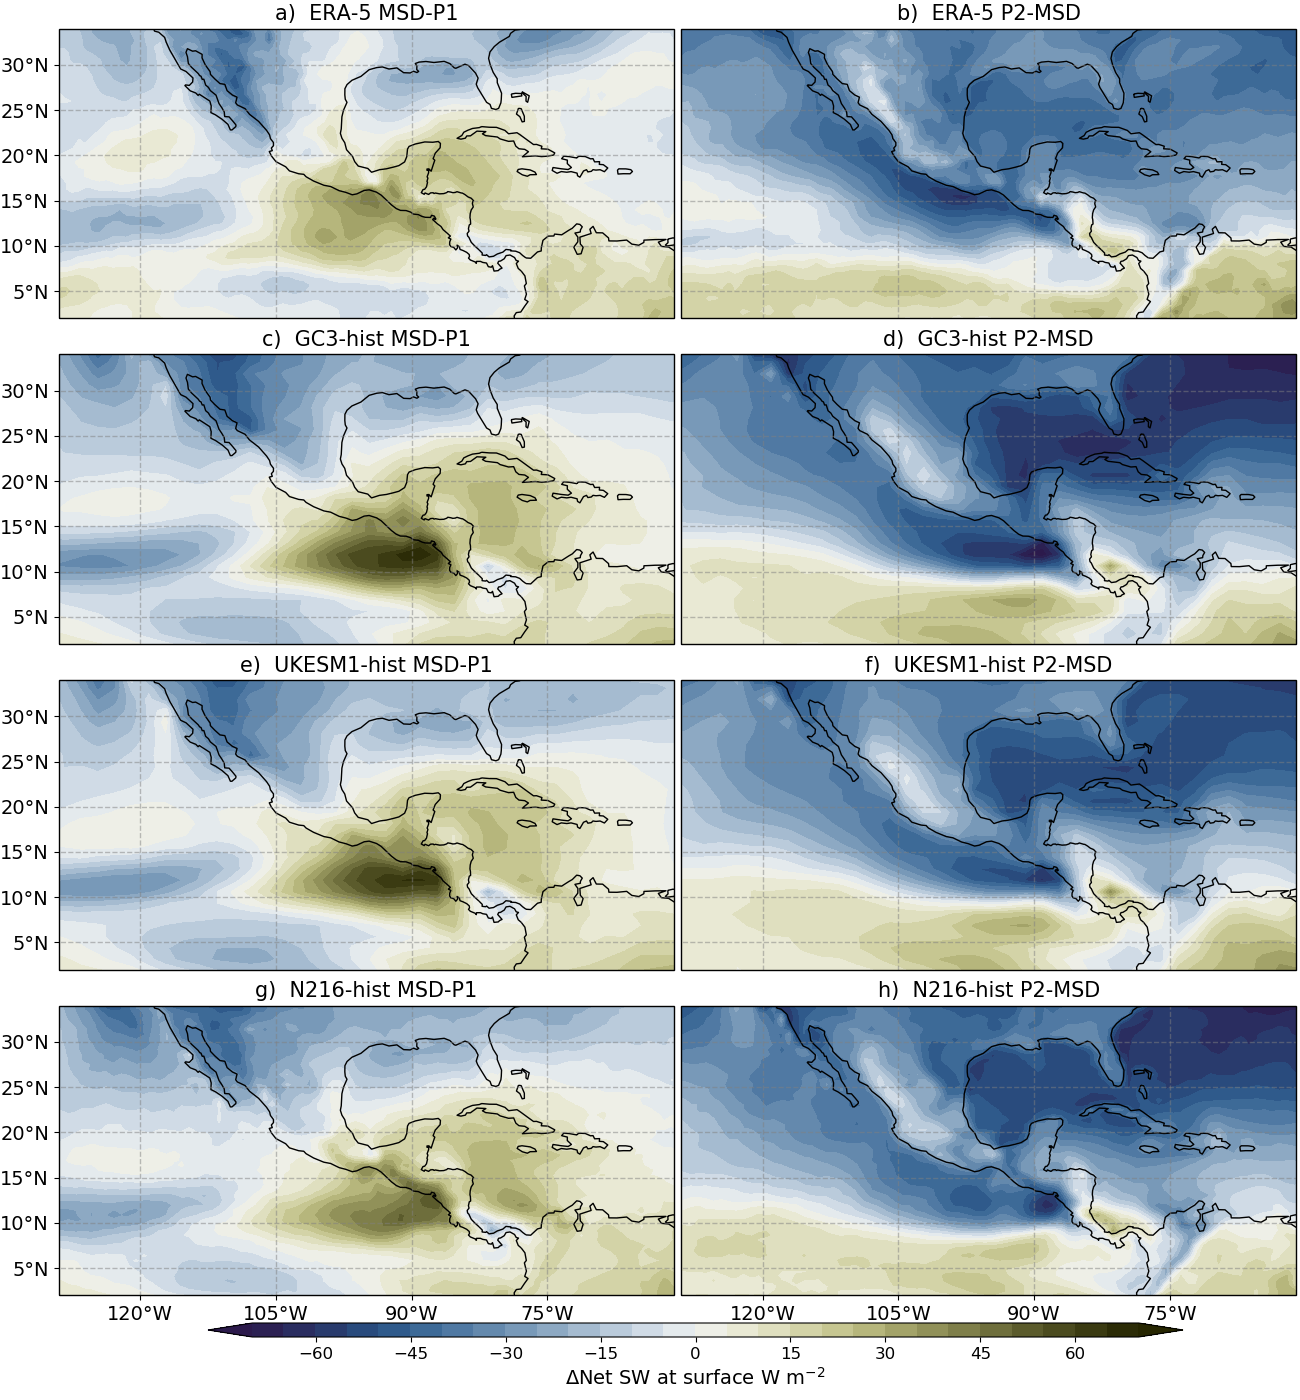
\includegraphics[width=\linewidth]{figures/fig4_netswdif_3.png}
\caption{As in Fig. \ref{fig:olranom}, but for the  net shortwave radiation [W m$^{-2}$] at the surface.}
\label{fig:swnet_diff}
\end{figure}

The spatial distribution of the composite mean changes to the net SW absorbed by the surface (Figure \ref{fig:swnet_diff}) show that from the first peak to the MSD there is a positive absorption of SW energy (by the surface in the MSD region of about 30 W m$^{-2}$ in ERA5 and 40 W m$^{-2}$. In contrast, for the P2-MSD differences, a notable reduction in net SW energy is observed throughout the North American continent.

One might reasonably then suspect that the increased SW absorption during the MSD may be the cause for the second peak of precipitation, as suggested by both \cite{magana1999} and \cite{karnauskas2013}. 

\begin{figure}[t!]
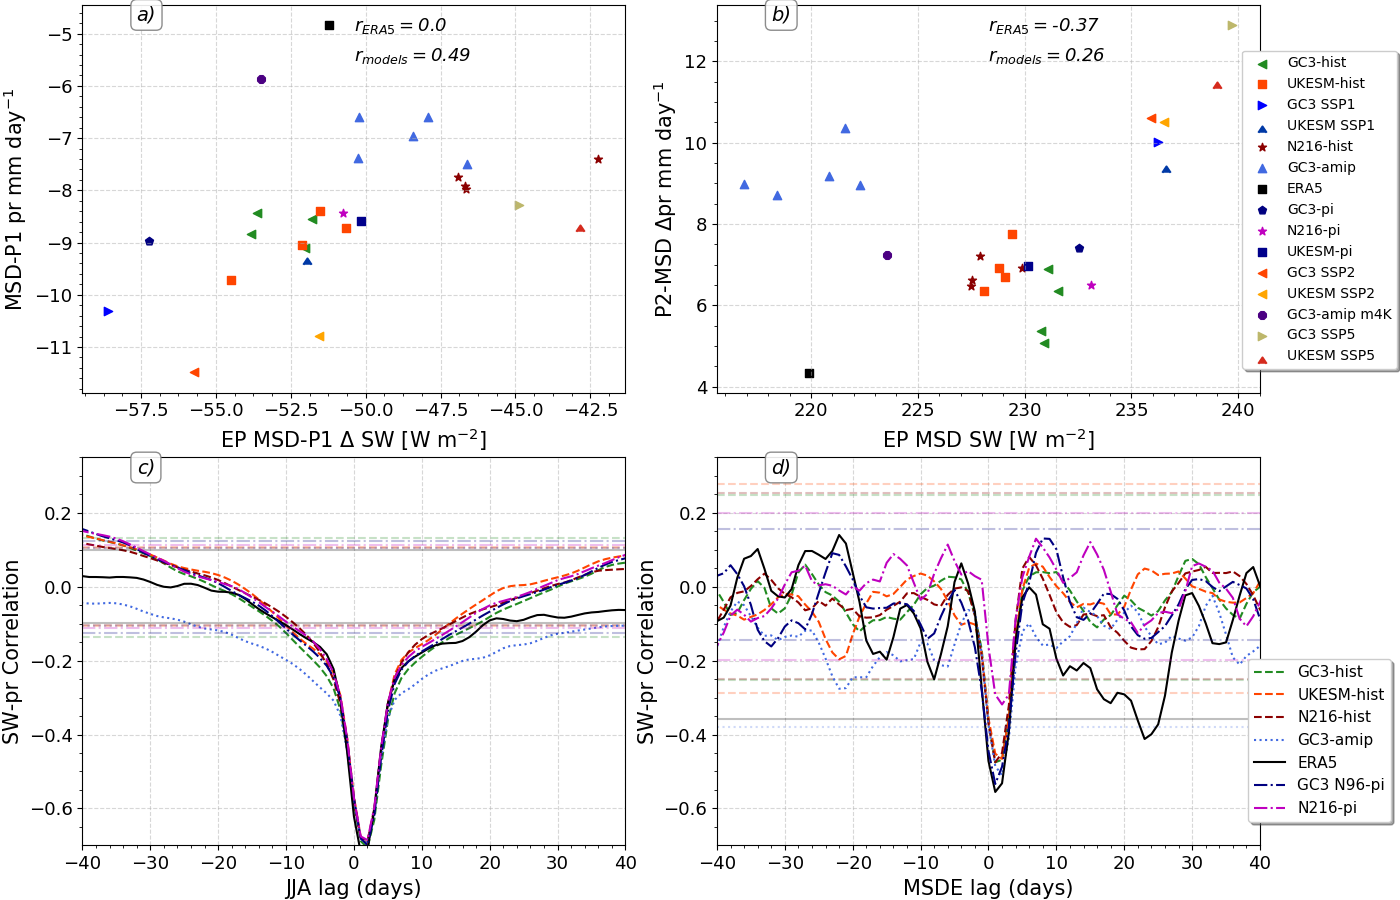
\includegraphics[width=\linewidth]{figures/cloud_scatter_f.png}
\caption{Scatter of .}
\label{fig:cloud_scatter}
\end{figure}


%For example, the Atlantic ITCZ biases have been shown to be directly affected by processes in the convective scheme \citep{bellucci2010}, such as the treatment of entraintment and moisture-cloud feedbacks \citep{oueslati2013,li2014}.

 
\begin{figure}[t!]
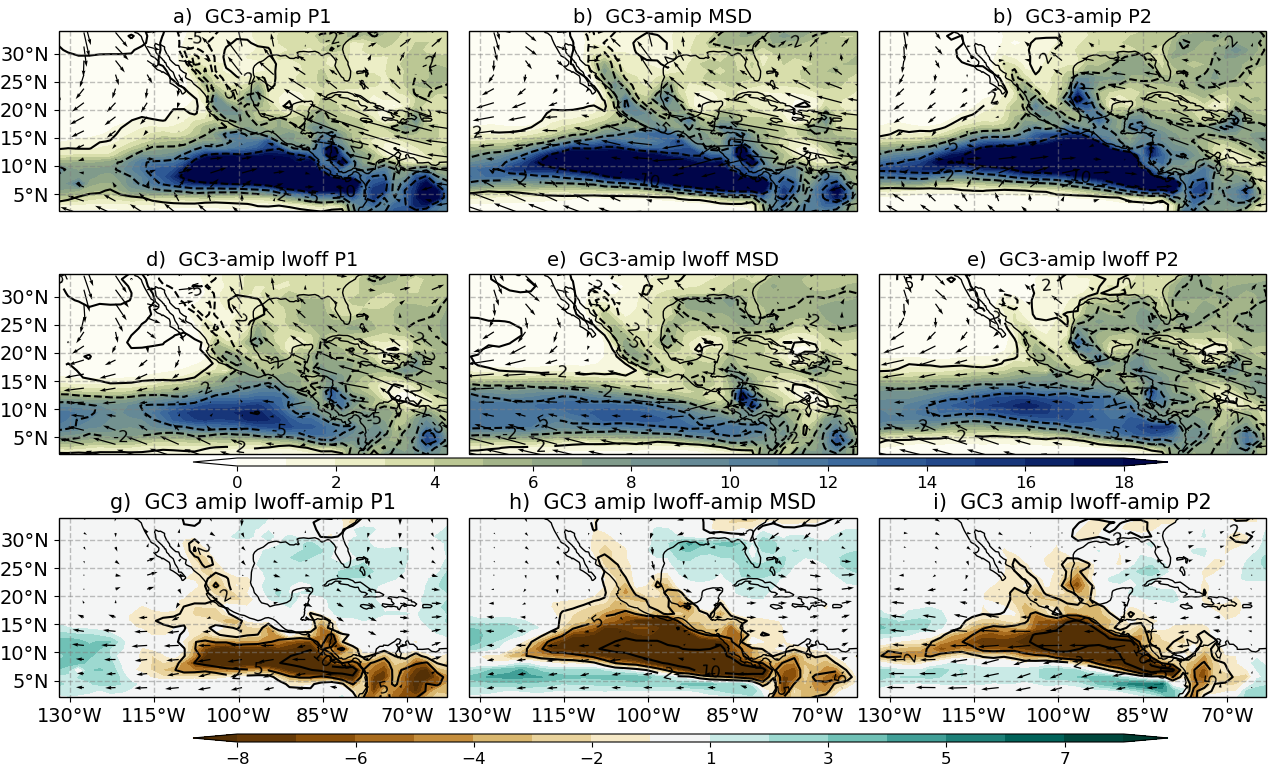
\includegraphics[width=\linewidth]{figures/lwfig_clim_1.png}
\caption{Composite mean precipitation (shading), vertical velocity (contours) and 850 hPa wind speed (vectors) for the P1, MSD and P2 periods in the (a-c) GC3-amip and (d-f) GC3-amip lwoff experiment. (g-i) shows the difference between the lwoff-amip and the amip experiments.}
\label{fig:lwoff}
\end{figure}

Finally, while the incoming SW has an important role in theories for the MSD, the LW effects have important consequences in general monsoon dynamics. 
The GC3-amip lwoff experiment is part of the Cloud Feedbacks MIP (CFMIP) is identical to the GC3-amip experiment except that the treatment of the LW in the radiation code in the model is not affected by the presence of clouds, in other words all LW fluxes are assumed to be under clear-sky conditions. 

The impact of the LW CRE for precipitation in the Mesomerican region is critical (Figure \ref{fig:lwoff}). When the LW effects of clouds are ignored, precipitation over the whole domain is greatly reduced (50-80\%), ascent becomes weaker and the low-level circulation also weakens. 
These results are in agreement with previous studies \citep{guo2015,byrne2020} that show that cloud radiative heating weakens the local and regional circulation in a monsoon. However, these LW appear to be stronger during the MSD and P2 periods than during the P1 period. 





\subsection{On the role of the Caribbean Low-Level Jet}

 \begin{figure}[t!]
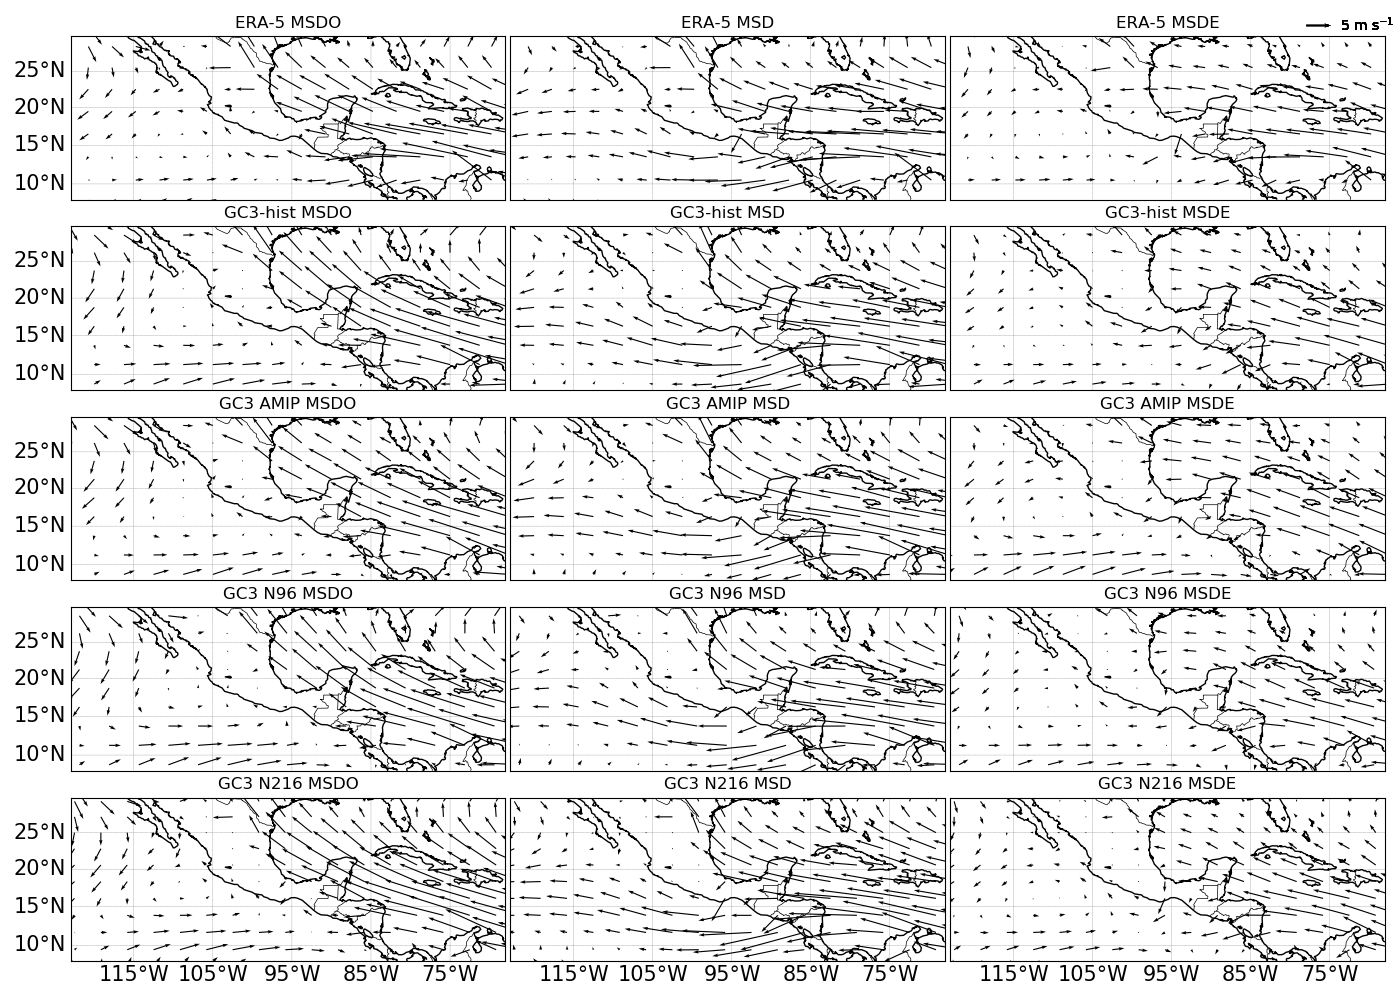
\includegraphics[width=\linewidth]{figures/modcompar_dif2u3}
\caption{As in Figure \ref{fig:msdolranom} but showing wind vectors at the 850 hPa level. }
\label{fig:msduanom}
\end{figure}


 \begin{figure}[t!]
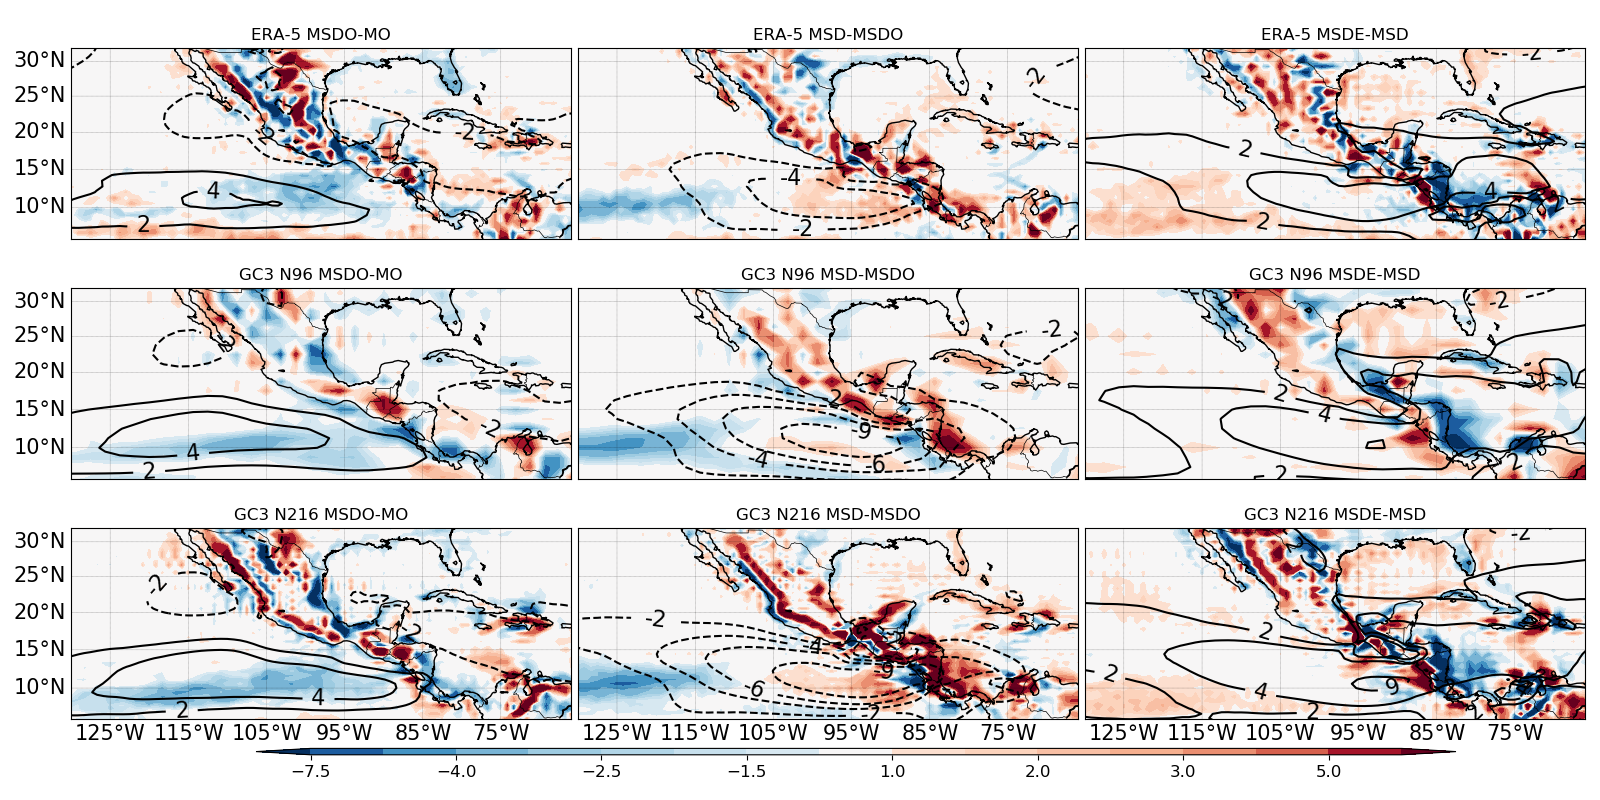
\includegraphics[width=\linewidth]{figures/modcompar_dif2mfc3}
\caption{As in Figure \ref{fig:msdolranom} but showing in shading, moisture flux divergence $\nabla \cdot \vec{u}q$ at the 850 hPa level with units of $10^{-7}$ s$^{-1}$ kg / kg and zonal wind anomalies (line contours) in m s$^{-1}$.  }
\label{fig:msdmfcanom}
\end{figure}

After the MSD, the western coast of the Baja California Peninsula continues to warm and the East Pacific continues to cool, in contrast to previous suggestions \citep{magana1999,magana2005,herrera2015}. Meanwhile, the Caribbean Sea warms by 1 K and the northern Gulf of Mexico slightly cools down. The incoming shortwave differences show a regional-scale decrease in incoming shortwave, as the summer draws to an end. 
These SST differences indicate that the meridional SST gradient in both the EP and Caribbean Sea and Gulf of Mexico is greatly modified during the stages of the MSD. 




%Composites prior to the onset of the MSD, during the MSD and after the MSDE were computed for several diagnostic variables. The periods were separated using the WT method to determine the dates of the MSDO and MSDE in ERA5 and the climate model output.
%Figure \ref{fig:msdolranom} shows the composite differences between the period of the MSD and of the two peaks in outgoing long-wave radiation (OLR) and vertical velocity ($\omega-500$) at 500 hPa.
%The positive OLR and $\omega$ anomalies in the MSD-MSDO panels in southern Mexico and northern Central America are indicative of decreased height of convection and decreased ascent, in agreement with the MSD being the drier period. These positive anomalies in the continent are accompanied by negative OLR and $\omega-500$ anomalies west of the continent, . 
%These anomalies are stronger in the simulations (e.g., Figure \ref{fig:msdolranom}c). 


%The MSDE-MSD panels show the difference between the second peak of rainfall and the drier MSD period. Negative OLR and $\omega$ anomalies indicate stronger and higher convection over a wide region including the easternmost Pacific Ocean, southern Mexico, northern Central America Cuba and the Caribbean Sea.  
%Note also the region of the North American Monsoon, on the northwest corner of Mexico and the southernmost US, as the MSD-MSDO difference suggests increased convective activity in the North American Monsoon region and 
%MSDE-MSD the opposite. 

 

%Similarly, Figure \ref{fig:msduanom} shows the low-level wind field during the three stages of the MSD. In ERA-5, prior to the MSD the wind flow in the Caribbean shows strong easterlies that flow into the Gulf of Mexico and southeastern US but very weak winds in the EP (see Figure \ref{fig:csst}f). During the MSD, the winds in the EP become modestly strong eaterlies associated the easterly flow from the Caribbean Sea that crosses over Costa Rica and Nicaragua from the Caribbean Sea to the East Pacific. Note that the easterlies converge towards the region at 125$^\circ$W where OLR and $\omega$ anomalies suggest increased ascent. 

%By the end of the MSD the easterlies in ERA5 weaken substantially on the western coast of Central America and in the Caribbean Sea.
%The simulations seem to generally reproduce the characteristics of the wind field with some differences worth mentioning. For instance, prior to the onset of the MSD, all the simulations show a modest westerly wind flow in the east Pacific at 10$^\circ$N, which can also be seen in Figure \ref{fig:csst}f, which is not observed in ERA5.
%After the MSD ends, most simulations show a very weak westerly flow in the East Pacific, close to ERA5; however, GC3 AMIP shows a modest westerly wind converging towards the west coast of Nicaragua. This low-level convergence may be forcing the increased convective activity and precipitation during this time in GC3 AMIP.

%The SSTs and incoming shortwave radiation are key elements for explain the seasonal cycle of the MSD, according to previous theories summarised in section \ref{sq:lit}. 
%Figure \ref{fig:msdsstanom} shows the corresponding SST and incoming shortwave anomalies during the different stages of the seasonal cycle. % MSD-MSDO and MSDE-MSD anomalies. 
%From the first peak to the MSD, a positive SST difference of +1.5 K in the Gulf of California and the western coast of the Baja California Peninsula is observed in reanalysis and the models. The differences appear as a sharp SST meridional gradient pattern around 115$^\circ$W. 
%During this stage, the incoming shortwave increases in Central America, which agrees with Figure \ref{fig:csst}d. 
%Note the negative incoming shortwave differences west of Central America at 125$^\circ$W, the region of negative OLR and $\omega$-500 hPa anomalies where low-level winds converge, all of which supports the notion of increased convective activity that reduces incoming shortwave west of the continent. This feature was noted by \cite{herrera2015}. 



The main dynamical argument put forth to explain the MSD is centred around variations in the moisture flux convergence (MFC), argued to be driven by the Caribbean-Low Level Jet \citep[see e.g.][]{gamble2008,herrera2015,martinez2019}. The MFC and zonal wind variations in each stage of the MSD is shown in Figure \ref{fig:msdmfcanom} for ERA-5 and two simulations. The low-level MFC increases from monsoon onset (MO) to the first peak period (MSDO) in the EP. This anomaly in MFC corresponds to a region of positive zonal wind anomalies indicative of weaker easterly flow.
 This zonal wind anomaly from MSD to MSDO is much stronger in the models.  
The MSD-MSDO difference shows a strong positive MFC anomaly across southern Mexico and most of Central America. 

In turn, the MFC anomalies associated with the end of the drier period, observed as the MSDE-MSD anomalies,  show negative values, suggesting increased moisture flux, over southern Mexico and northern Central America.
Increased moisture flux during the transition from the MSD to the second peak agrees well with the precipitation differences during these periods.  The MSDE-MSD zonal wind anomalies in the EP show positive zonal wind anomalies, suggesting a weakened easterly wind flow (see also Fig. \ref{fig:msduanom}). 

The MSD in Central America and southern Mexico has been strongly linked to the strengthening of the CLLJ \citep{herrera2015}. The maximum zonal wind observed in the CLLJ is found at the very end of July (Fig. \ref{fig:csst}e), synchronized with the start of the MSD. 
The zonal wind anomalies in the MSD-MSDO panels in Figure \ref{fig:msdmfcanom} show that easterlies in the Caribbean Sea do not strengthen by more than 2 m s$^{-1}$ from the first peak to the MSD. Only in the models is there a modest negative anomaly at the westernmost Caribbean Sea. In other words, while the peak of the climatological CLLJ coincides with the climatological timing of the onset of the MSD, these composite analyses constructed by more specifically separating the MSD periods does not show relevant variations in the zonal wind of the Caribbean Sea. 
The drier MSD period does coincide with stronger easterly flow over the eastern Pacific, which may be associated with the weaker MFC over land. %The end of the MSD then coincides when the easterly winds weaken. 

\subsection{A look at the MSD through the lense of the moist static energy budget}

\section{Summary and discussion}\label{sq:sumdiscuss}


 \begin{figure}[t!]
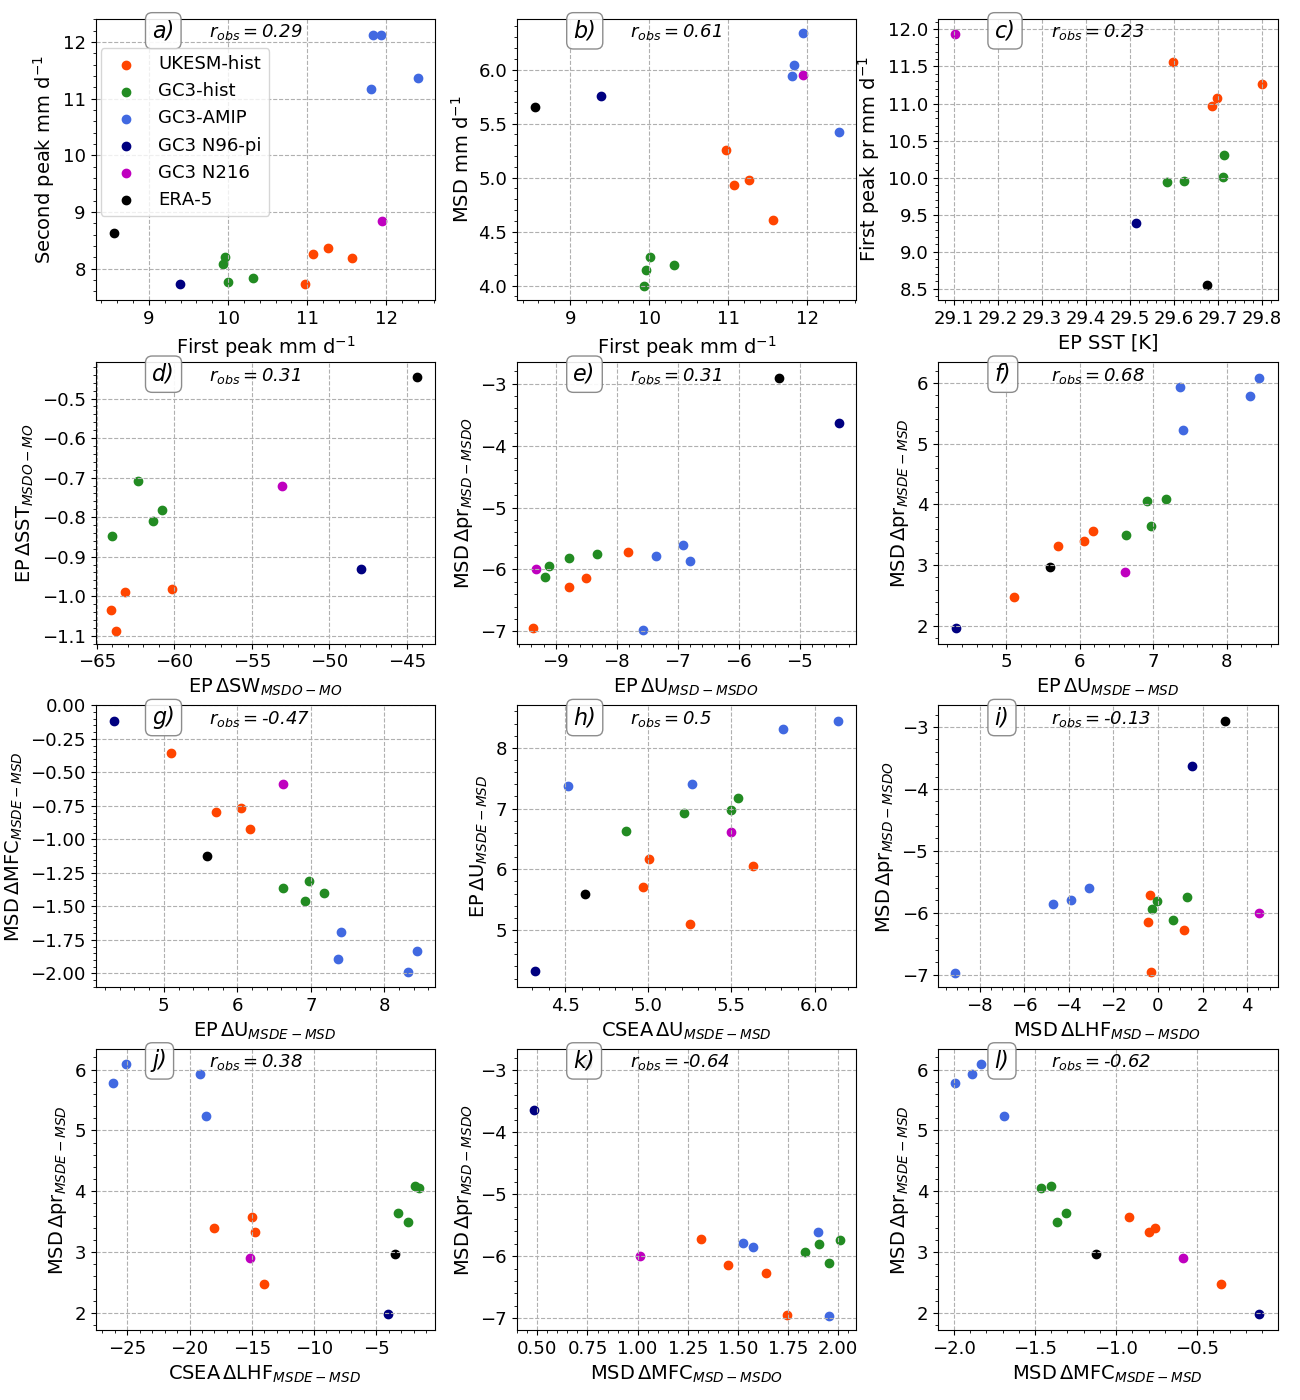
\includegraphics[width=\linewidth]{figures/scatter}
\caption{Scatter plot of the (a, b) area-averaged precipitation over land  (Box in Figure \ref{fig:7}) during the different stages of the MSD. (c) scatter of the East Pacific SSTs against  the precipitation over landduring the first peak period. (d-l) show the scatter differences in several variables between the different stages of onset of the MSD (MSDO), the drier MSD and the end of the MSDE. The differences are shown for area-averaged quantities in the East Pacific (EP), the Caribbean Sea (CSEA) and overland (MSD) as above. The units for $\Delta$U are [m s$^{-1}$], $\Delta$MFC [10$^{-11}$ s$^{-1}$], $\Delta$SW and $\Delta$LHF [W m$^{-2}$] and $\Delta$pr mm d$^{-1}$.   The Pearson correlation coefficient for the 38 yr of  reanalysis or observations ($r_{obs}$) is shown for each panel. }
\label{fig:scatter}
\end{figure}

The midsummer drought  is a  prominent feature of the seasonal cycle of rainfall of southern Mexico, northern Central America and the Caribbean. The average 20\%  decrease during the midsummer compared to the wetter periods of early and late summer is a rare feature of monsoon regions that has important implications for agriculture and water management  \citep{hellin2017,de2018,harvey2018}. 

Climate predictions of the MSD, particularly those concerning whether this "drought" will become more pronounced in the following years, are not trustworthy because of several reasons. 
One factor is the current limitation in the understanding of the physical processes that cause the MSD (section \ref{sq:lit}) as debate still exists over which large or regional-scale processes are most important to explain the increases and decreases of precipitation over intraseasonal time-scales.
Secondly, methods used to diagnose the timing and strength of the MSD typically deal with monthly-scale metrics, which would obscure subtle trends and processes that have an effect on shorter time-scales. 
Also relevant is the fact that climate models used to produce the predictions show significant biases in the EP ITCZ and the seasonal cycle of rainfall in the region, in fact, most CMIP3 and CMIP5 models did not show a bimodal signature in the seasonal cycle. Models that do not have a climatological MSD cannot provide a prediction for this regime in future climate. 

For these reasons, this section analysed the CMIP6 simulations from the Met Office models, UKESM1 and HadGEM3, aiming to understand the causes of the biases in the seasonal cycle. Furthermore, these models are better compared to CMIP3 and CMIP5 cohorts since UKESM1 and HadGEM3 actually simulate a bimodal precipitation regime in these regions. 
The purpose of this investigation is to use these climate models to better diagnose the relevant biases for the representation of the MSD but also understand the processes that these models are capturing leading to the MSD, in order to, hopefully, also highlight the dynamics of the MSD in general. 
%Therefore,this section and future thesis chapter evaluates the similarities and differences between reanalysis and model experiments. 
% For varios reasons, determining the timing and strength of the MSD is very important to agricultural practices,  and water management planning. 





%The different experiments showed notable differences in the precipitation amount in the MSD seasonal cycle.  The first peak, however, appears to be modestly related  to the precipitation amount during the MSD in the models and in observations ($r=0.6$) suggesting that the wetter the first peak the wetter the MSD period.  


 The wavelet transform method was developed to determine the pentads of onset and end of the MSD.  For instance, Figures \ref{fig:scatter}a,b show the scatter of the mean precipitation during the first peak against second peak and first peak against MSD in all the simulations and ERA5. The magnitude of the first and second peaks appear to be unrelated in these models and in observations, which would suggest that the processes driving each peak are not exactly the same.
 Similarly, composite analysis of various diagnostics during the different stages of the seasonal cycle was done, for instance,  OLR composites showed that the MSD is not a local feature in a small region of southern Mexico but extends throughout a wide range of North America,  from central Mexico through Belize, Guatemala, El Salvador, Honduras, Nicaragua, and northern Costa Rica. % Although the MSD has been documented in all these regions \citep{magana1999,perdigon2018}, these composites showed a synchronicity in the precipitation anomalies and a larger extent to the western Mexican coastline that were not previously shown, to our knowledge. OLR anomalies between the second peak and the MSD also showed a simultaneous increased convective activity in the Caribbean. 
 
 This composite approach also allowed to test previously proposed hypotheses by analysing the differences between model experiments and the observed variability in the characteristics of the precipitation at each stage of the MSD.
 For example, \cite{magana1999} proposed a mechanism that explains the MSD through SST-cloud feedbacks. In this hypothesis, shortwave, SSTs and precipitation are strongly coupled in the EP Ocean. The first peak of precipitation in southern Mexico and Central America would then be associated with the EP SSTs prior to the onset of rainfall. 
 Figure \ref{fig:scatter}c shows that EP SSTs prior to onset do not explain the inter-model differences in the magnitude of the first peak nor do they show a strong relationship in the observed interannual variability of the first peak mean precipitation. 
 Similarly, Figure \ref{fig:scatter}d shows that surface incoming shortwave variations are only weakly related to SSTs variations in the EP, in both models and reanalysis, during the first peak period. 
 
The feedback mechanism also suggests that the second peak is a result of a second increase in surface incoming shortwave that occurs as cloud cover decreases during the drier MSD. This increase in incoming shortwave then increases EP SSTs and thus increasing convective activity. Although the incoming shortwave does show a bimodal behaviour (Figure \ref{fig:csst}d), the SSTs in the East Pacific do not increase during the MSD period, but in fact cool during the end of the MSD.   Furthermore, as in Figure \ref{fig:scatter}d, variations in incoming shortwave were not strongly related to SST changes in any of the stages of the MSD (not shown). This suggests that the SSTs are not only dependent on the incoming shortwave in both models and reanalysis.

The low-level winds (Figure \ref{fig:msduanom}) show notable changes between the onset of the MSD (MSDO), the MSD and the end of the MSD (MSDE).
  Weak westerlies in the EP are found during the wetter periods but the zonal wind becomes a modest easterly flow during the drier MSD period. 
  The MSDO appears to be synchronized with the strengthening of the Caribbean Low-Level Jet (Fig. \ref{fig:csst}e). During the MSD, the strong zonal flow in the Caribbean crosses Central America into the central-eastern Pacific. This easterly flow during the MSD converges to 125$^\circ$W in the EP Ocean, a region that also shows increased ascent during the MSD. 
 % The zonal wind the East Pacific seems to be modulated by the wind in the Caribbean Sea, i.e., by the Caribbean Low-Level Jet strength.
 
Figure \ref{fig:scatter}e, f show the relationships between the zonal flow in the EP Ocean and precipitation in southern Mexico and Central America. 
The changes in the wind flow between the first and the MSD are not related to the drying response over land during the same period. 
However, the differences between the second peak and the MSD in the wind flow and precipitation show a strong relationship both in observed interannual variability as well as in the model spread. Simulations with a stronger EP zonal wind anomaly show the strongest increment in precipitation over land.
The zonal wind change in the EP from the MSD to the second peak period is also modestly related to the MFC over the continent (Fig. \ref{fig:scatter}g) with weaker easterly winds in the EP associated with more convergence over land in the models and reanalysis. 


%is associated with the variability observed in the precipitation changes from the MSD to the second peak, as well as with the MFC in the MSD region.  
The easterly flow in the EP has been associated with the strength of the CLLJ \citep{herrera2015}. The zonal wind changes in the MSDE-MSD difference in the EP shows a modest linear relationship with the zonal flow in the Caribbean Sea (Fig. \ref{fig:scatter}h). During the other periods, the relationship between the CLLJ and the EP zonal component of the wind is even weaker in both models and observations (not shown). 

%However, the zonal wind in the Caribbean Sea is not linearly related to MFC in the MSD region (panel g). In other words, it appears the CLLJ influences the EP zonal flow but not the MFC or precipitation in the MSD directly. 
 
A potentially relevant bias found in the models was stronger-than-observed surface latent heat fluxes (LHF) (Figure \ref{fig:csst}g, h) compared to the reanalysis.  Changes in the surface energy balance and the surface temperature in historical versus pre industrial control simulations may also be responsible for the precipitation differences between these experiments.  However, the variations in the LHFs, both MSD-MSDO and MSDE-MSD either in the Caribbean Sea or over land (Figure \ref{fig:scatter}i,j) are not related to precipitation over land.



The main factor associated with the precipitation variations in the seasonal cycle appears to be the low-level moisture flux convergence (MFC) (Figure \ref{fig:scatter}k, l). The variations in the MFC over land explain intermodel differences and observed interannual variability in precipitation, particularly in the positive rainfall increment from the MSD to the second peak. From the first peak to the MSD, moisture flux decreases and increases again from the MSD to the second peak. % The lowest decrease Stronger moisture flux into region leads to   
 
